\documentclass[dvipdfmx]{jsarticle}
\usepackage[dvipdfmx]{graphicx}
\usepackage{caption}
\usepackage{here}
\captionsetup[figure]{labelsep=period, labelfont=bf, justification=raggedright, singlelinecheck=off}

\begin{document}
    \begin{titlepage}
        \begin{center}
            \vspace*{180truept}
            {\Huge 技術書SNS 設計書}

            \vspace{160truept}
            {\Large グループメンバー}
            %なんか書かないといけないので適当に役割書いてます

            \vspace{20truept}
            {\Large バックエンド担当 \quad20-1-037-0112 穂積 優真}

            \vspace{10truept}
            {\Large フロントエンド担当 20-1-037-0027 實藤 敬太}
            {\Large }

            \vspace{160truept}
            \today
        \end{center}
    \end{titlepage}
    \newpage

    \section*{イントロダクション}
    \subsection*{\rm{作成者:穂積(バックエンド担当)}}
    \section{アプリケーションの目的}
    本アプリケーションの目的は, 以下のとおりである.
    \begin{itemize}
        \item 読んだ技術書についての情報や個人的な感想などを投稿して,知識の整理や獲得をする
        \item 他のユーザとコミュニケーションをとる
    \end{itemize}

    \section{アプリケーションの範囲}
    本アプリケーションは, 「技術書SNS」と呼び, SNSサービスを提供する.

    SNSとは, タイムライン上にテキストやマルチメディアデータを用いた投稿を行い, 他のユーザとの間でのコミュニケーションを促進するためのサービスであり, 次に挙げるような機能を持っている.

    \begin{itemize}
        \item タイムライン機能
        \item プロフィール機能
        \item メッセージ送受信機能
        \item ユーザ相互リンク機能
        \item ユーザ検索機能
        \item コミュニティ機能
        \item ログイン認証機能
    \end{itemize}

    \section{アプリケーションの概要}
    本アプリケーションは, 技術書の共有をテーマにしたSNSサービスを提供するものである. 本アプリケーションのユーザは, 次に挙げる機能を使用することができる.

    \begin{itemize}
        \item アカウントの新規登録
        \item アカウント認証
        \item 技術書に関する投稿
        \item タイムライン上の投稿の閲覧
        \item 投稿に対するコメント
        \item 技術書の検索
    \end{itemize}

    \section{アプリケーションの条件}
    本アプリケーションに課された条件は, 以下のとおりである.
    \begin{itemize}
        \item 2023/1/11までに本アプリケーションを完成させること
        \item 本アプリケーションは, WARファイルで提供すること
        \item WARファイルのみを配備すれば, 任意のサーブレットコンテナ上で実行可能なこと
    \end{itemize}
    \newpage

    \section*{ユースケース図とユースケース記述}
    \subsection*{\rm{作成者:穂積(バックエンド担当)}}
        \begin{figure}[H]
            \begin{center}
                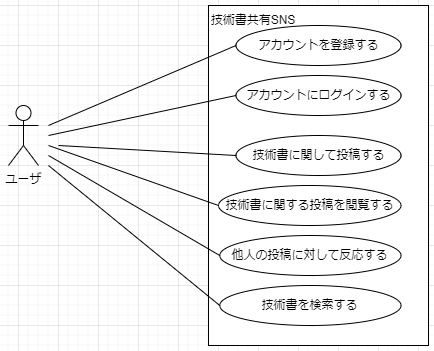
\includegraphics[scale=1.0,clip]{pictures/usecase.drawio_1.png}
            \end{center}
        \end{figure}
    \newpage

    \subsection*{\rm{作成者:ユースケース記述 穂積(バックエンド担当)}}
    \begin{table}[H]
        \begin{tabular}{|l|l|} \hline
            ユースケース名 & アカウントを登録する          \\ \hline
            アクター    & ユーザ                 \\ \hline
            事前条件    &   1. Webブラウザが起動されている.  \\ \hline
            基本系列    & 
            \begin{tabular}{l}
                1. Webブラウザが起動されている. \\ 
                2.  システムが, ログイン用のページを表示する.\\
                3. アクターが「新規登録」ボタンを押下する.\\
                4. システムが, アカウント登録用のページを表示する.\\
                5. アクターが「Username」フィールドにユーザ名を入力する.\\
                6. アクターが「Password」フィールドにパスワードを入力する.\\
                7. アクターが「送信」ボタンを押下する.\\
                8. システムが, 送信されたユーザの情報をアクターの新規アカウントとして記録する.\\
                9. システムが, ログイン用のページを表示する.
            \end{tabular} \\\hline
            事後条件    &   
            \begin{tabular}{l}
                1. アクターの新規アカウントが記録されている.\\
                2. ログイン用のページが表示されている.
            \end{tabular}
            \\ \hline
            説明      & 
            \begin{minipage}{140mm} 
                \vspace{4truept}
                1. ログイン用のページ
                \begin{itemize}
                    \item 本アプリケーションのタイトルを表示する.
                    \item ユーザ名を入力するための「Username」フィールドを表示する.
                    \item パスワードを入力するための「Password」フィールドを表示する.
                    \item 入力したユーザ情報でログインするための「ログイン」ボタンを表示する.
                    \item アカウントを新規登録するための「新規登録」ボタンを表示する
    
                \end{itemize}
                2. アカウント登録用のページ
                \begin{itemize}
                    \item ユーザ名を入力するための「Username」フィールドを表示する.
                    \item パスワードを入力するための「Password」フィールドを表示する.
                    \item 入力したユーザ情報を登録するための「送信」ボタンを表示する. 
                \end{itemize}
                \vspace{4truept}
            \end{minipage}
            
            \\ \hline
        \end{tabular}
    \end{table}

    \newpage


    \begin{table}[H]
        \begin{tabular}{|l|l|} \hline
            ユースケース名 & アカウントにログインする          \\ \hline
            アクター    & ユーザ                 \\ \hline
            事前条件    &   1. ログイン用のページが表示されている.  \\ \hline
            基本系列    & 
            \begin{tabular}{l}
                1. アクターが「Username」フィールドにユーザ名を入力する.\\
                2. アクターが「Password」フィールドにパスワードを入力する.\\
                3. アクターが「ログイン」ボタンを押下する.\\
                4. システムがメインページを表示する
            \end{tabular} \\\hline
            事後条件    &   1. メインページが表示されている.
            \\ \hline
            説明      & 
            \begin{minipage}{130mm} 
                \vspace{4truept}
                1. メインページ
                \begin{itemize}
                    \item 本アプリケーションのタイトルを表示する.
                    \item ユーザ全員の投稿をいくつか送信順に表示する
                    \item ユーザ自身のユーザ名を表示する
                    \item ユーザ自身のプロフィールを表示するための「プロフィール」ボタンを表示する
                    \item 技術書を検索するための「検索」ボタンを表示する.
                    \item 技術書に関する投稿をするための「投稿」ボタンを表示する.
                    \item 投稿に対するコメントを送信するための「コメントする」ボタンを表示する.
    
                \end{itemize}

                \vspace{4truept}
            \end{minipage}
            
            \\ \hline
        \end{tabular}
    \end{table}

    \newpage


    \begin{table}[H]
        \begin{tabular}{|l|l|} \hline
            ユースケース名 & 技術書に関して投稿する          \\ \hline
            アクター    & ユーザ                 \\ \hline
            事前条件    &   1. メインページが表示されている.  \\ \hline
            基本系列    & 
            \begin{tabular}{l}
                1. アクターが,「投稿」ボタンを押下する.\\
                2. システムが技術書投稿フォームを表示する.\\
                3. アクターが, 技術書に関する情報をフィールドに入力する.\\
                4. アクターが,「新規投稿」ボタンを押下する.\\
                5. アクターが, 送信された情報を技術書情報として記録する.\\
                6. システムが, メインページを表示する.
            \end{tabular} \\\hline
            事後条件    &   1. アクターが投稿した、技術書情報が記録されている.
            \\ \hline
            説明      & 
            \begin{minipage}{130mm} 
                \vspace{4truept}
                1. 技術書に関する情報
                \begin{itemize}
                    \item 書名
                    \item ISBN
                \end{itemize}

                
                2. 技術書投稿フォーム
                \begin{itemize}
                    \item 書名を入力するための「Title」フィールドを表示する.
                    \item ISBNを入力するための「ISBN」フィールドを表示する.
                    \item フォームを送信するための「新規投稿」ボタンを表示する.
                \end{itemize}
                \vspace{4truept}
            \end{minipage}
            
            \\ \hline
        \end{tabular}
    \end{table}

    \newpage

    \begin{table}[H]
        \begin{tabular}{|l|l|} \hline
            ユースケース名 & 技術書に関する投稿を閲覧する          \\ \hline
            アクター    & ユーザ                 \\ \hline
            事前条件    &   1. メインページが表示されている.  \\ \hline
            基本系列    & 1. システムが, メインページに表示されている技術書に関する投稿を更新する. \\\hline
            事後条件    &   1. メインページが表示されている.
            \\ \hline
            説明      & 
            \begin{minipage}{130mm} 
                \vspace{4truept}
                1. 技術書に関する投稿
                \begin{itemize}
                    \item ユーザ名と技術書に関する情報からなる組.
                \end{itemize}
                \vspace{4truept}
            \end{minipage}
            
            \\ \hline
        \end{tabular}
    \end{table}

    \newpage

    \begin{table}[H]
        \begin{tabular}{|l|l|} \hline
            ユースケース名 & 他人の投稿に対して反応する          \\ \hline
            アクター    & ユーザ                 \\ \hline
            事前条件    &   1. メインページが表示されている.  \\ \hline
            基本系列    & 
            \begin{tabular}{l}
                1. アクターが, 「コメント投稿」ボタンを押下する.\\
                2. システムが, コメント投稿フォームを表示する.\\
                3. アクターが, 「Comment」フィールドに送信するメッセージを入力する.\\
                4. アクターが, 「コメントする」ボタンを押下する.\\
                5. システムが, 送信されたコメントをアクターからの発言として記録する.\\
                6. システムが, メインページを表示する.
            \end{tabular} \\\hline
            事後条件    &   
            \begin{minipage}{130mm}
                \vspace{4truept}
                \begin{enumerate}
                    \item アクターからの発言が記録されている
                    \item メインページが表示されている
                \end{enumerate}
                \vspace{4truept}
            \end{minipage}

            \\ \hline
            説明      & 
            \begin{minipage}{130mm} 
                \vspace{4truept}
                1. 発言
                \begin{itemize}
                    \item ユーザ名とコメントからなる組
                \end{itemize}

                
                2. コメント投稿フォーム
                \begin{itemize}
                    \item 他の人の投稿に対して、感想を入力するための「Comment」フィールドを表示する.
                    \item フォームを送信するための「コメントする」ボタンを表示する.
                \end{itemize}
                \vspace{4truept}
            \end{minipage}
            
            \\ \hline
        \end{tabular}
    \end{table}

    \newpage

    \begin{table}[H]
        \begin{tabular}{|l|l|} \hline
            ユースケース名 & 技術書を検索する          \\ \hline
            アクター    & ユーザ                 \\ \hline
            事前条件    &   1. メインページが表示されている.  \\ \hline
            基本系列    & 
            \begin{tabular}{l}
                1. アクターが, 「検索」ボタンを押下する.\\
                2. システムが, 検索フォームを表示する.\\
                3. アクターが, 「Search」フィールドに検索ワードを入力する.\\
                4. アクターが「検索する」ボタンを押下する.\\
                5. システムがメインページを表示する.\\
                6. システムが検索条件に応じてタイムラインを更新する.
            \end{tabular} \\\hline
            事後条件    &   
            \begin{minipage}{130mm}
                \vspace{4truept}
                \begin{enumerate}
                    \item メインページが表示されている.
                    \item 検索条件によって、表示される投稿が絞られている
                \end{enumerate}
                \vspace{4truept}
            \end{minipage}

            \\ \hline
            説明      & 
            \begin{minipage}{130mm} 
                \vspace{4truept}
                1. 検索フォーム
                \begin{itemize}
                    \item 検索条件を入力するための「Search」フィールドを表示する.
                    \item フォームを送信するための「検索する」ボタンを表示する.
                \end{itemize}

                \vspace{4truept}
            \end{minipage}
            
            \\ \hline
        \end{tabular}
    \end{table}

    \newpage

    
    \section*{ページ遷移図}
    \subsection*{\rm{作成者:ユースケース記述 穂積(バックエンド担当)}}
    \begin{figure}[H]
        \begin{center}
            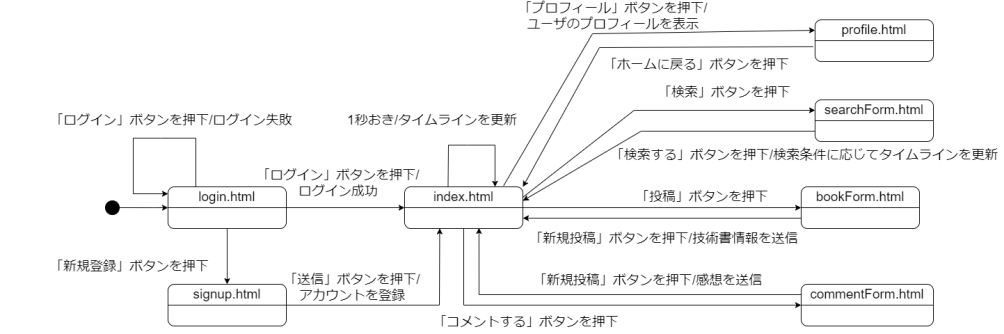
\includegraphics[scale=0.5,clip]{pictures/pageSenni_1.png}
        \end{center}
    \end{figure}

    

    \newpage

    \section*{試作ページ}
    \subsection*{\rm{作成者:穂積(バックエンド担当)\& 實藤(フロントエンド担当)}}
    \begin{figure}[H]
        \begin{center}
            \caption*{login.html}
            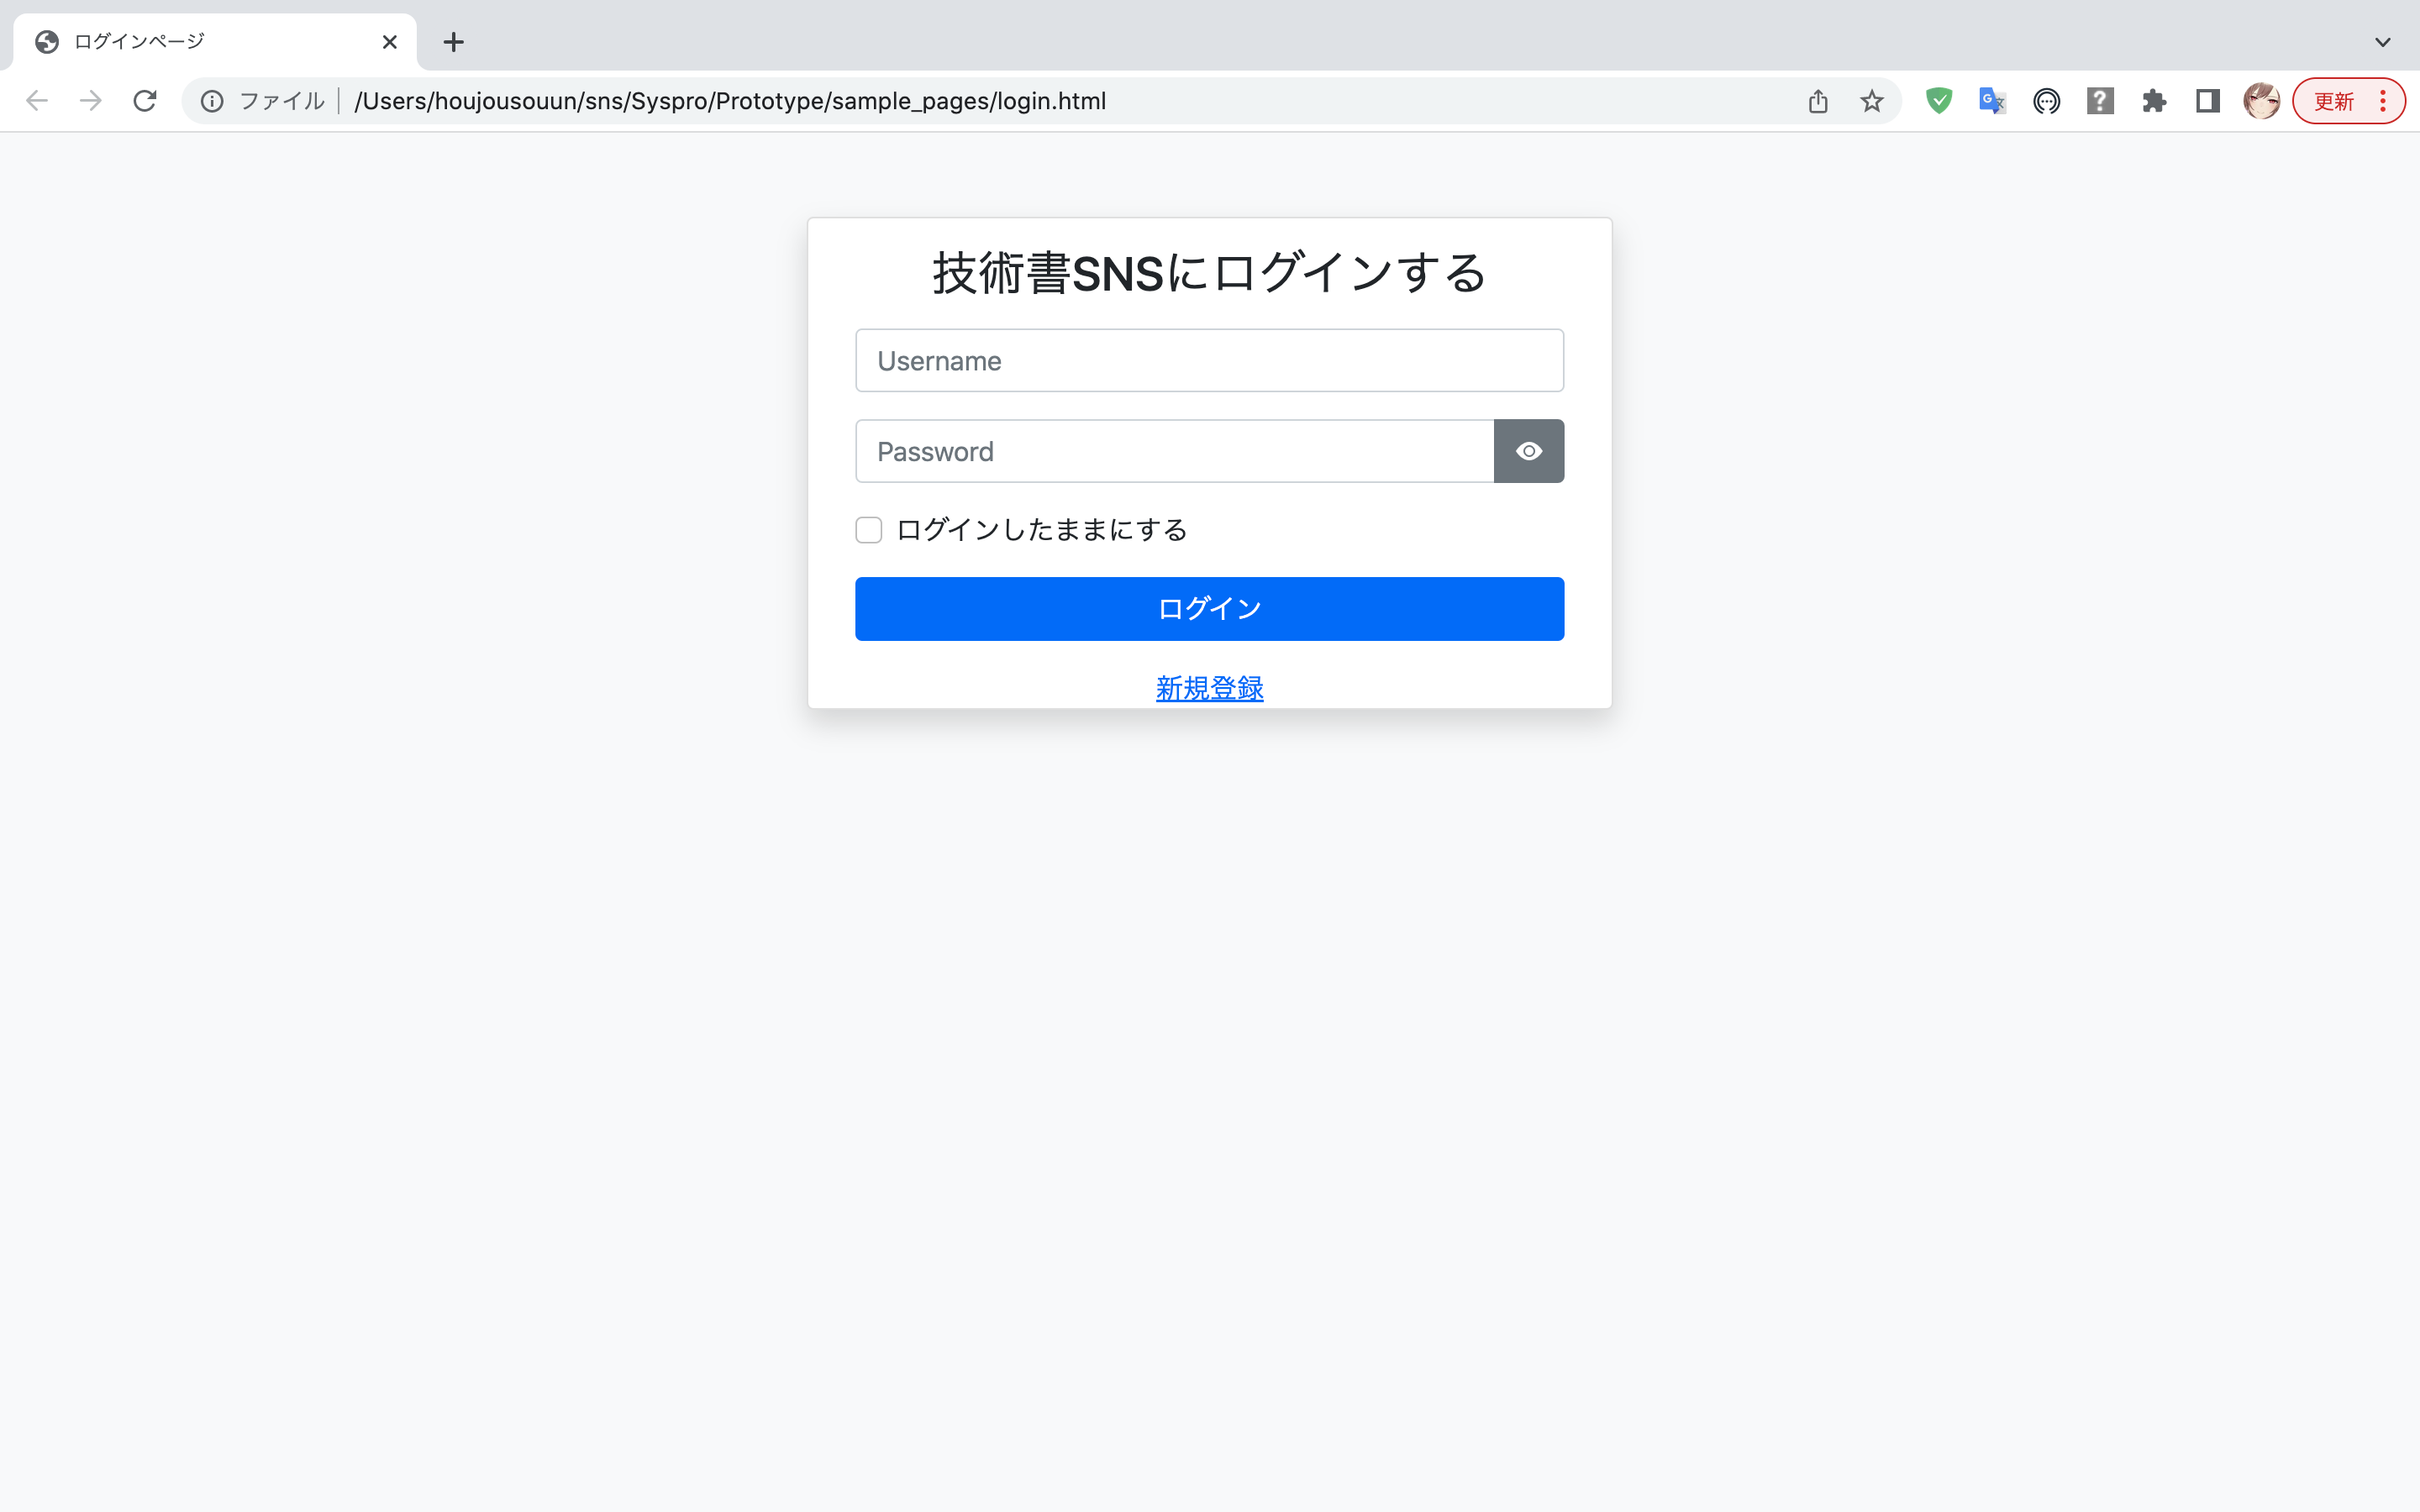
\includegraphics[scale=0.3,clip]{pictures/login.png}
        \end{center}
    \end{figure}

    \begin{figure}[H]
        \begin{center}
            \caption*{signup.html}
            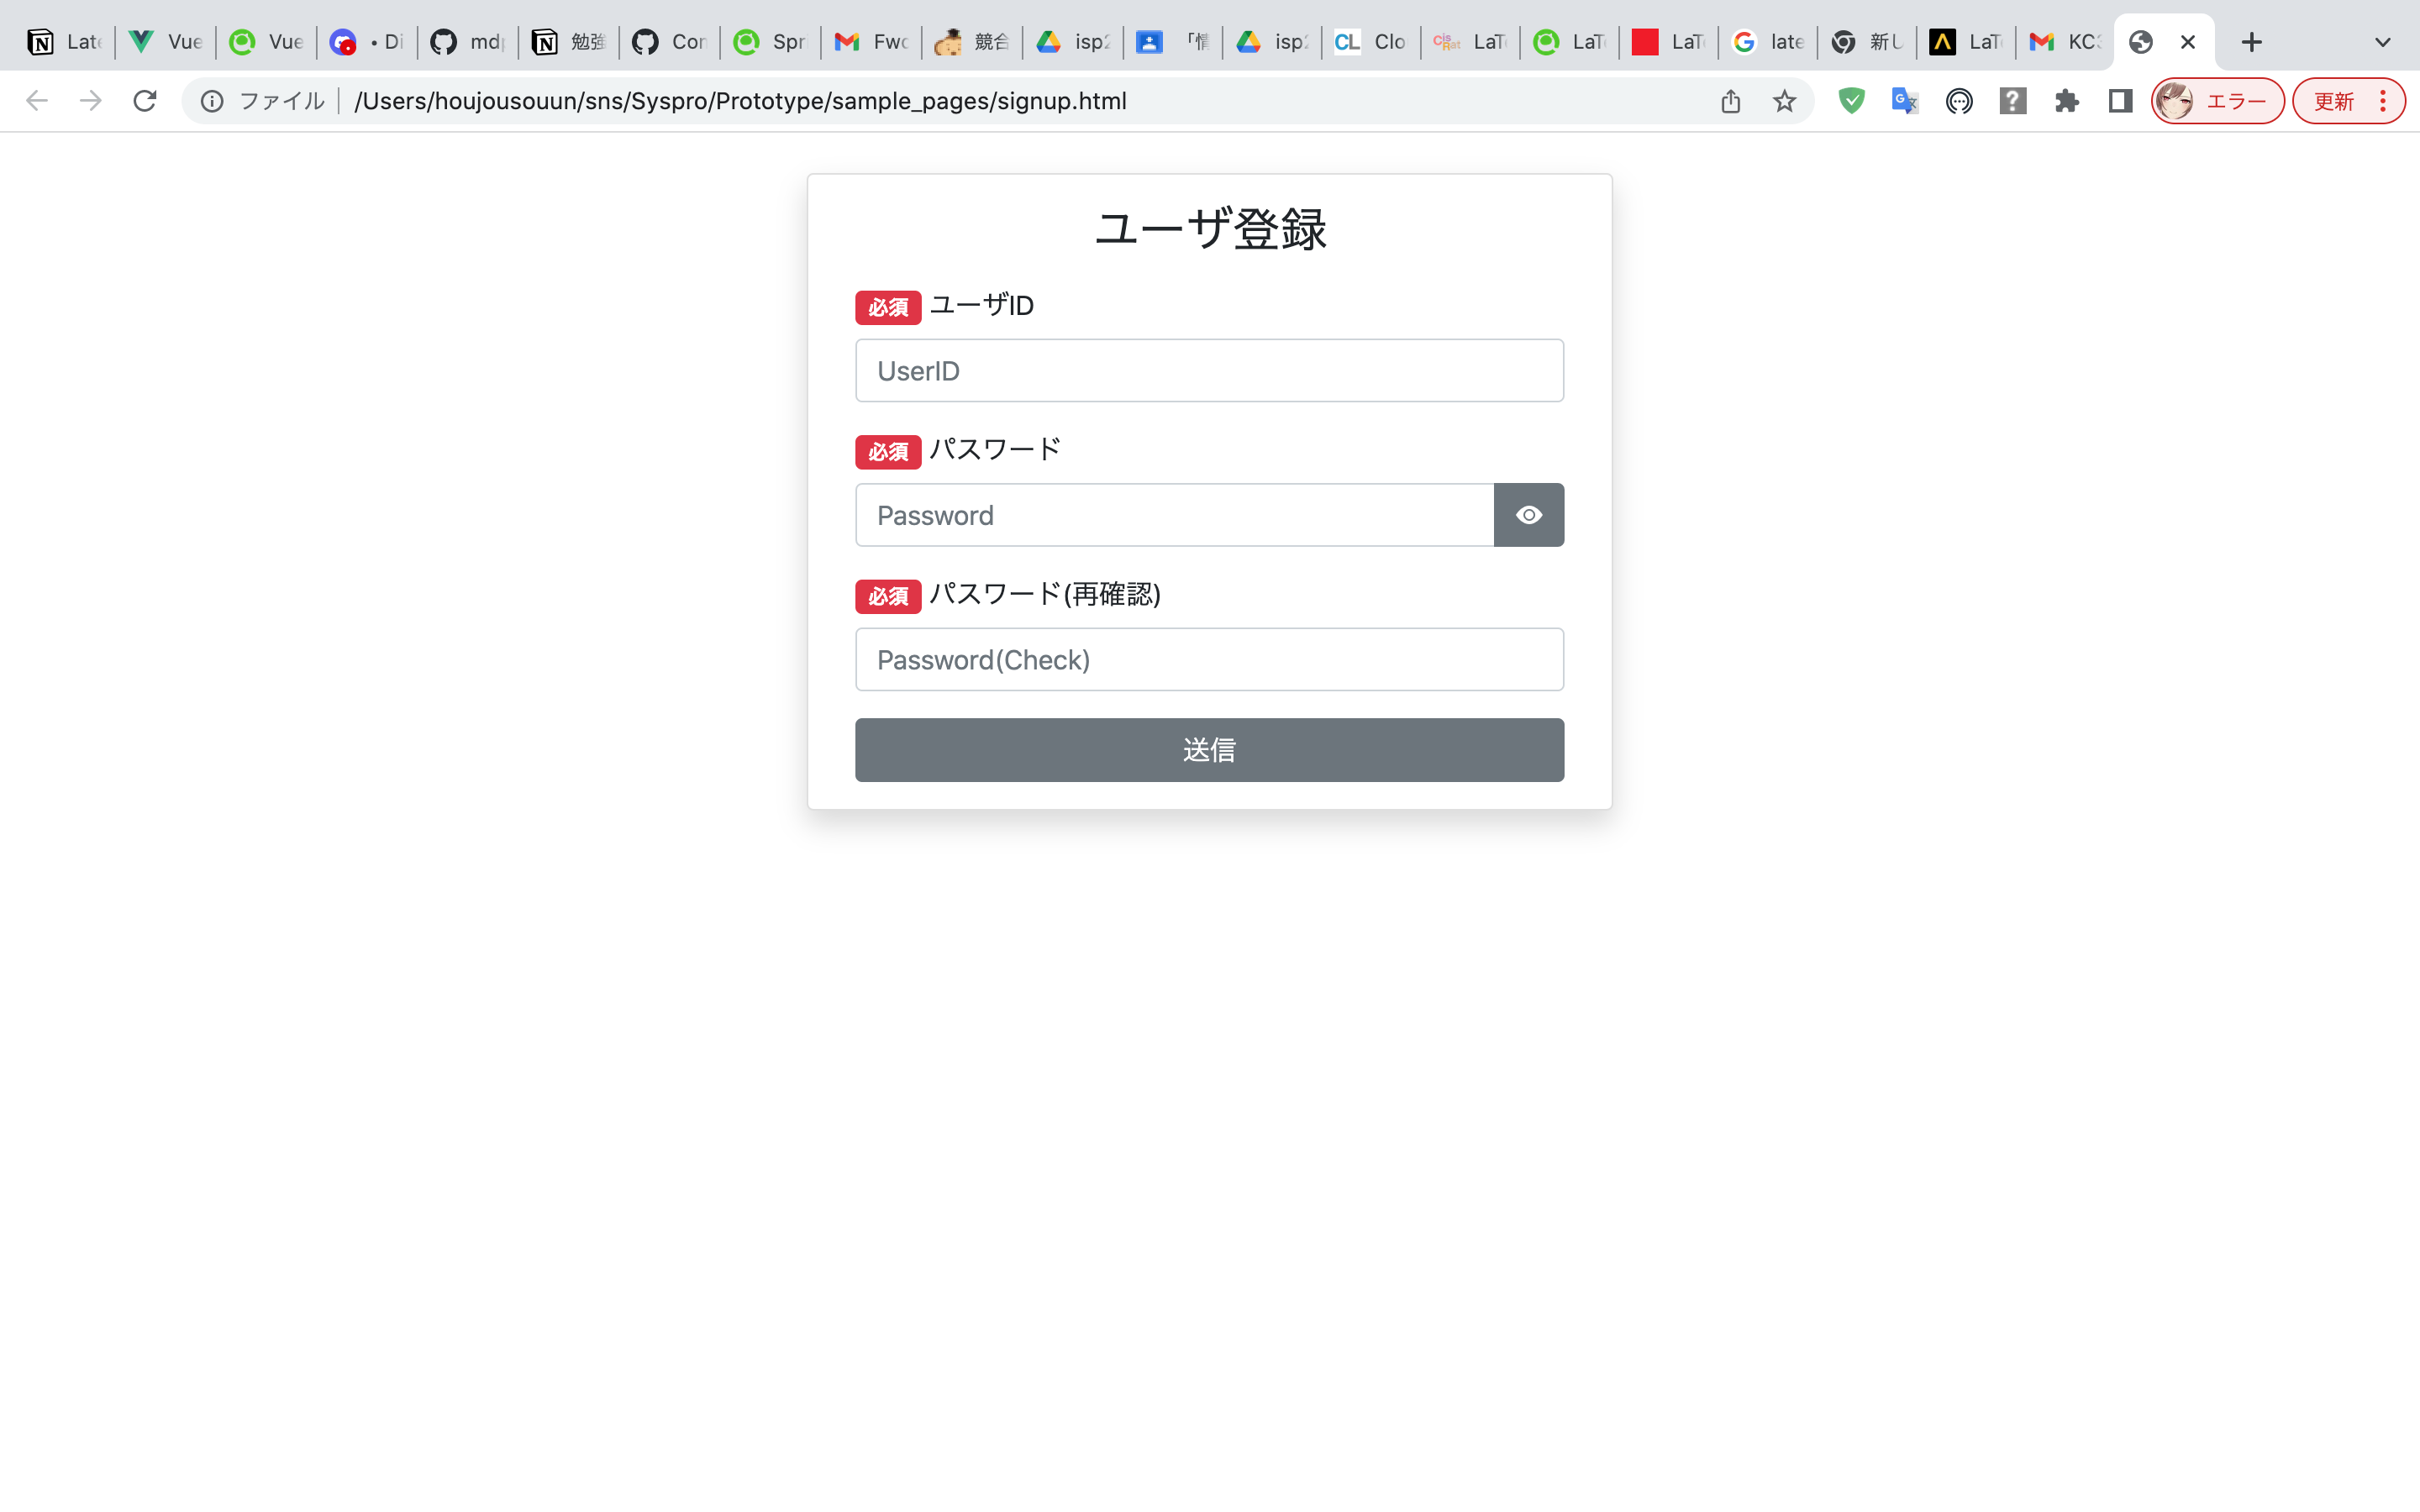
\includegraphics[scale=0.3,clip]{pictures/signup.png}
        \end{center}
    \end{figure}

    \begin{figure}[H]
        \begin{center}
            \caption*{index.html}
            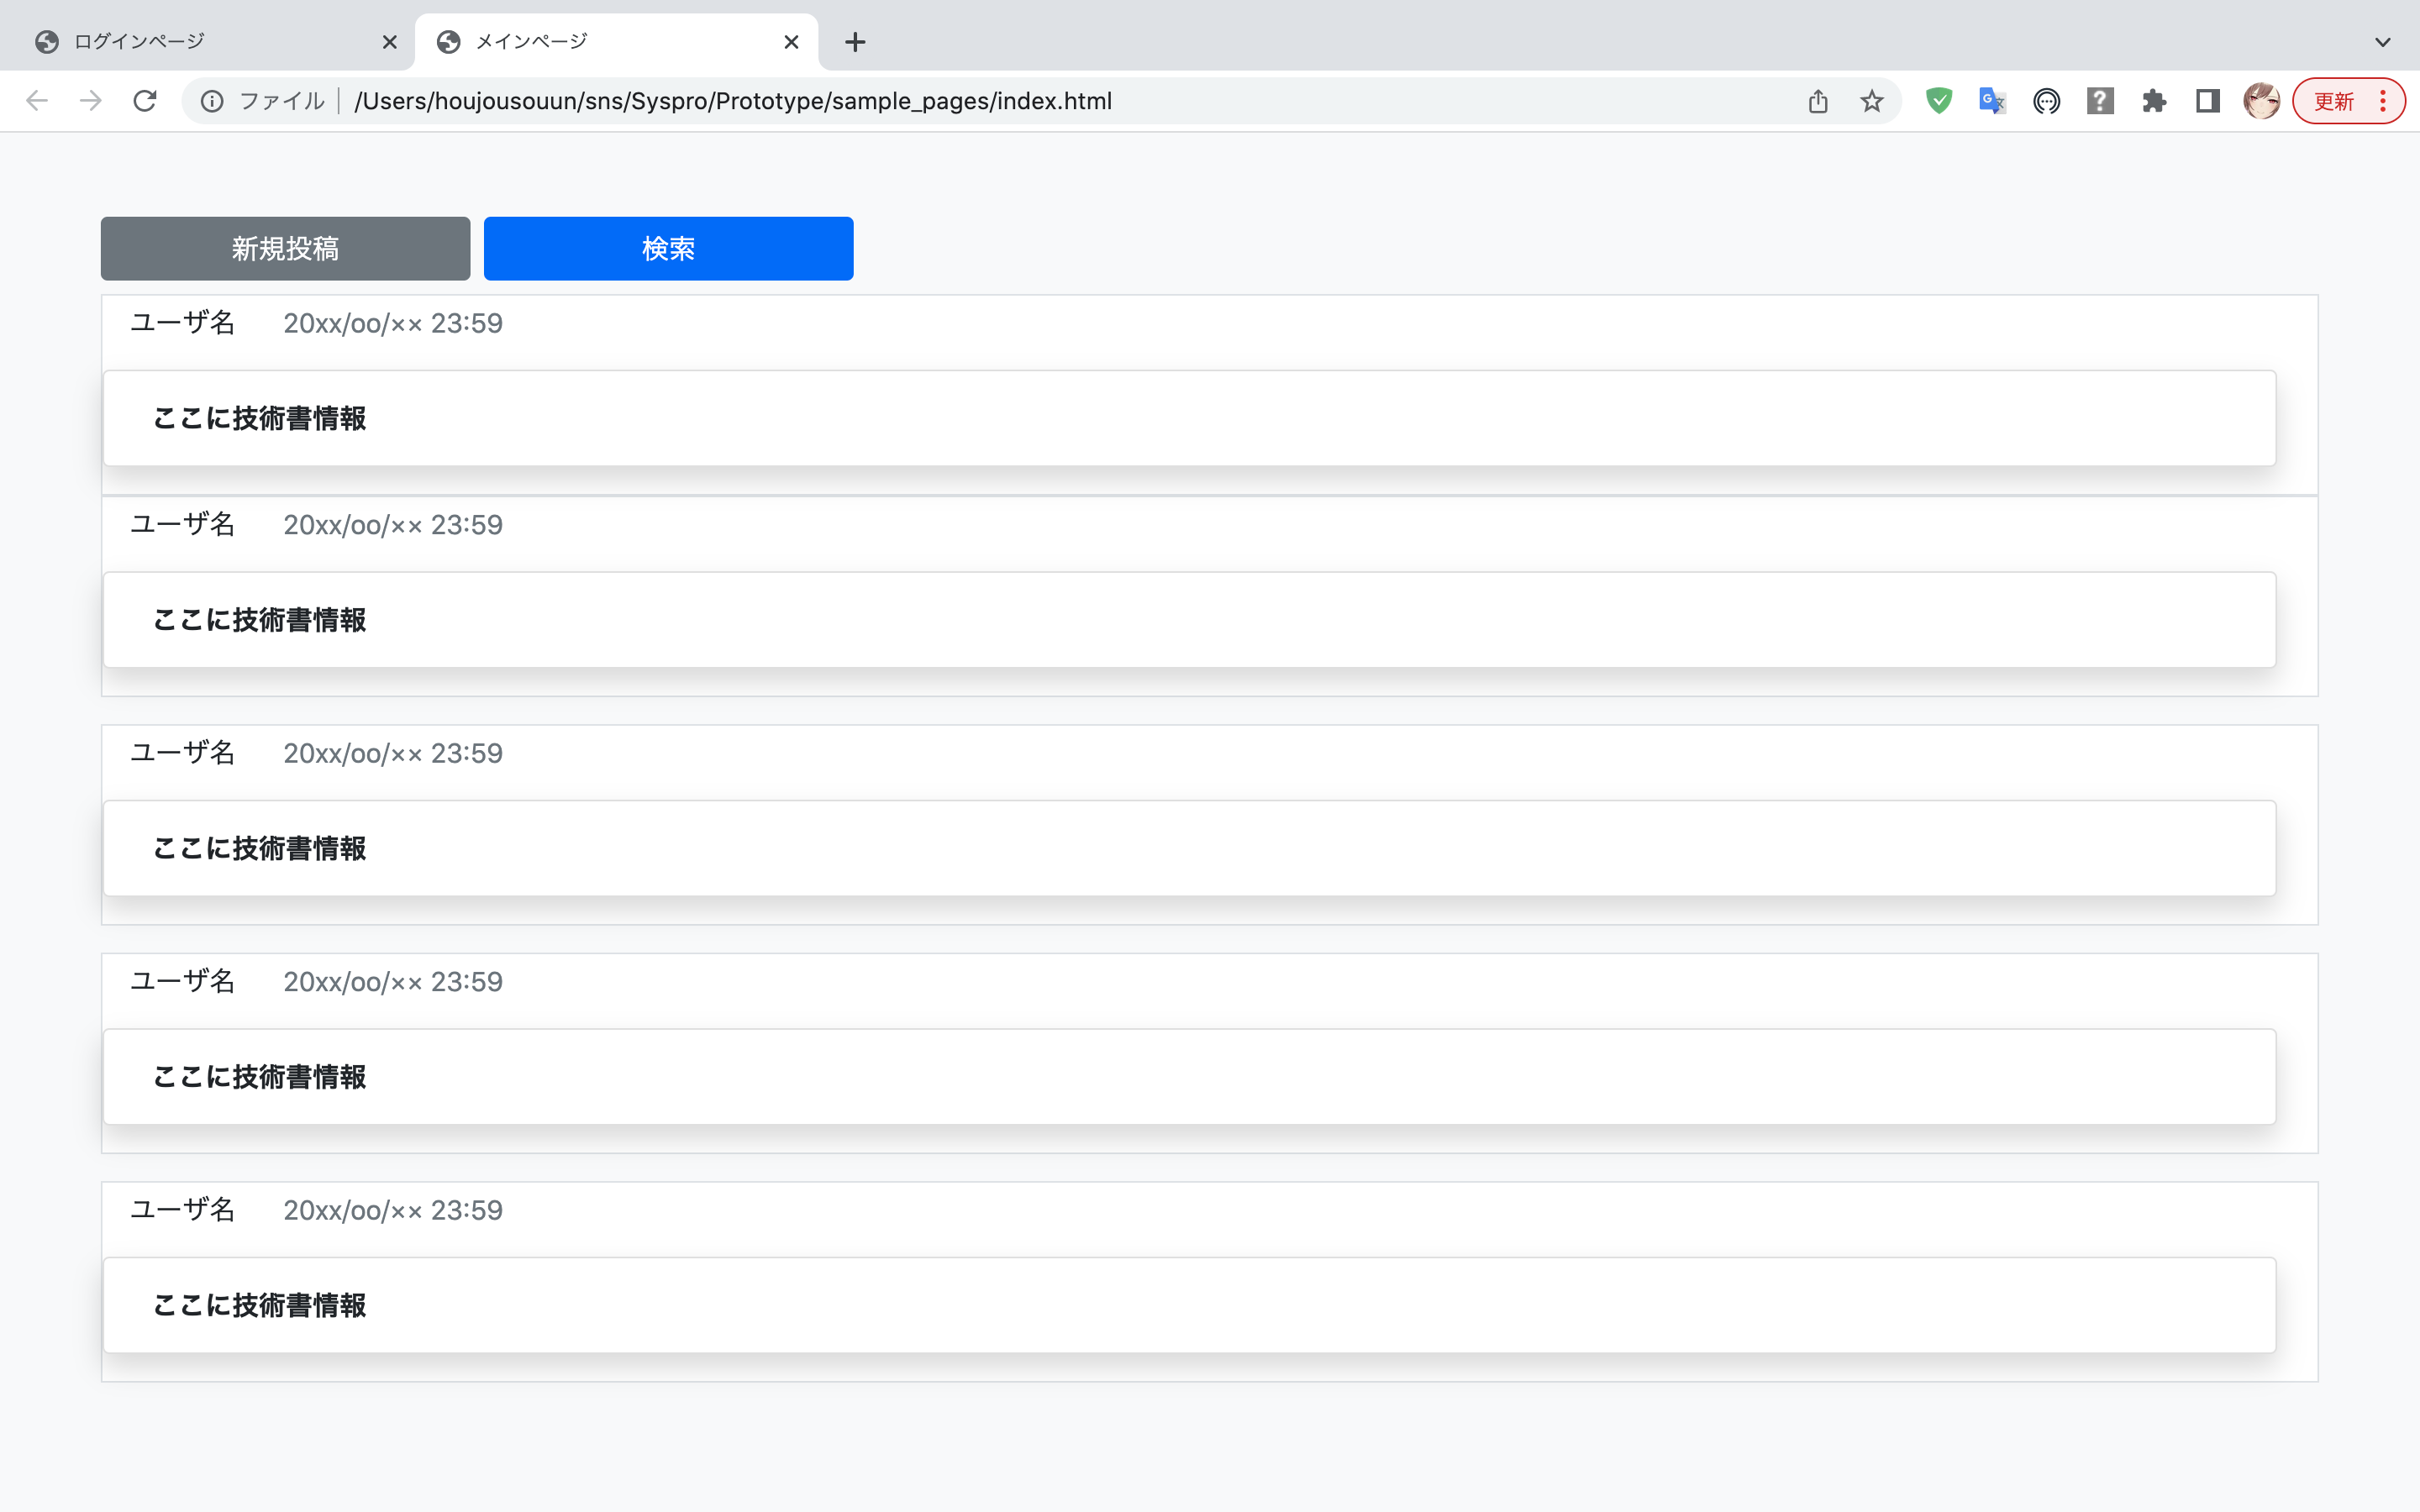
\includegraphics[scale=0.3,clip]{pictures/index.png}
        \end{center}
    \end{figure}

    \begin{figure}[H]
        \begin{center}
            \caption*{profile.html}
            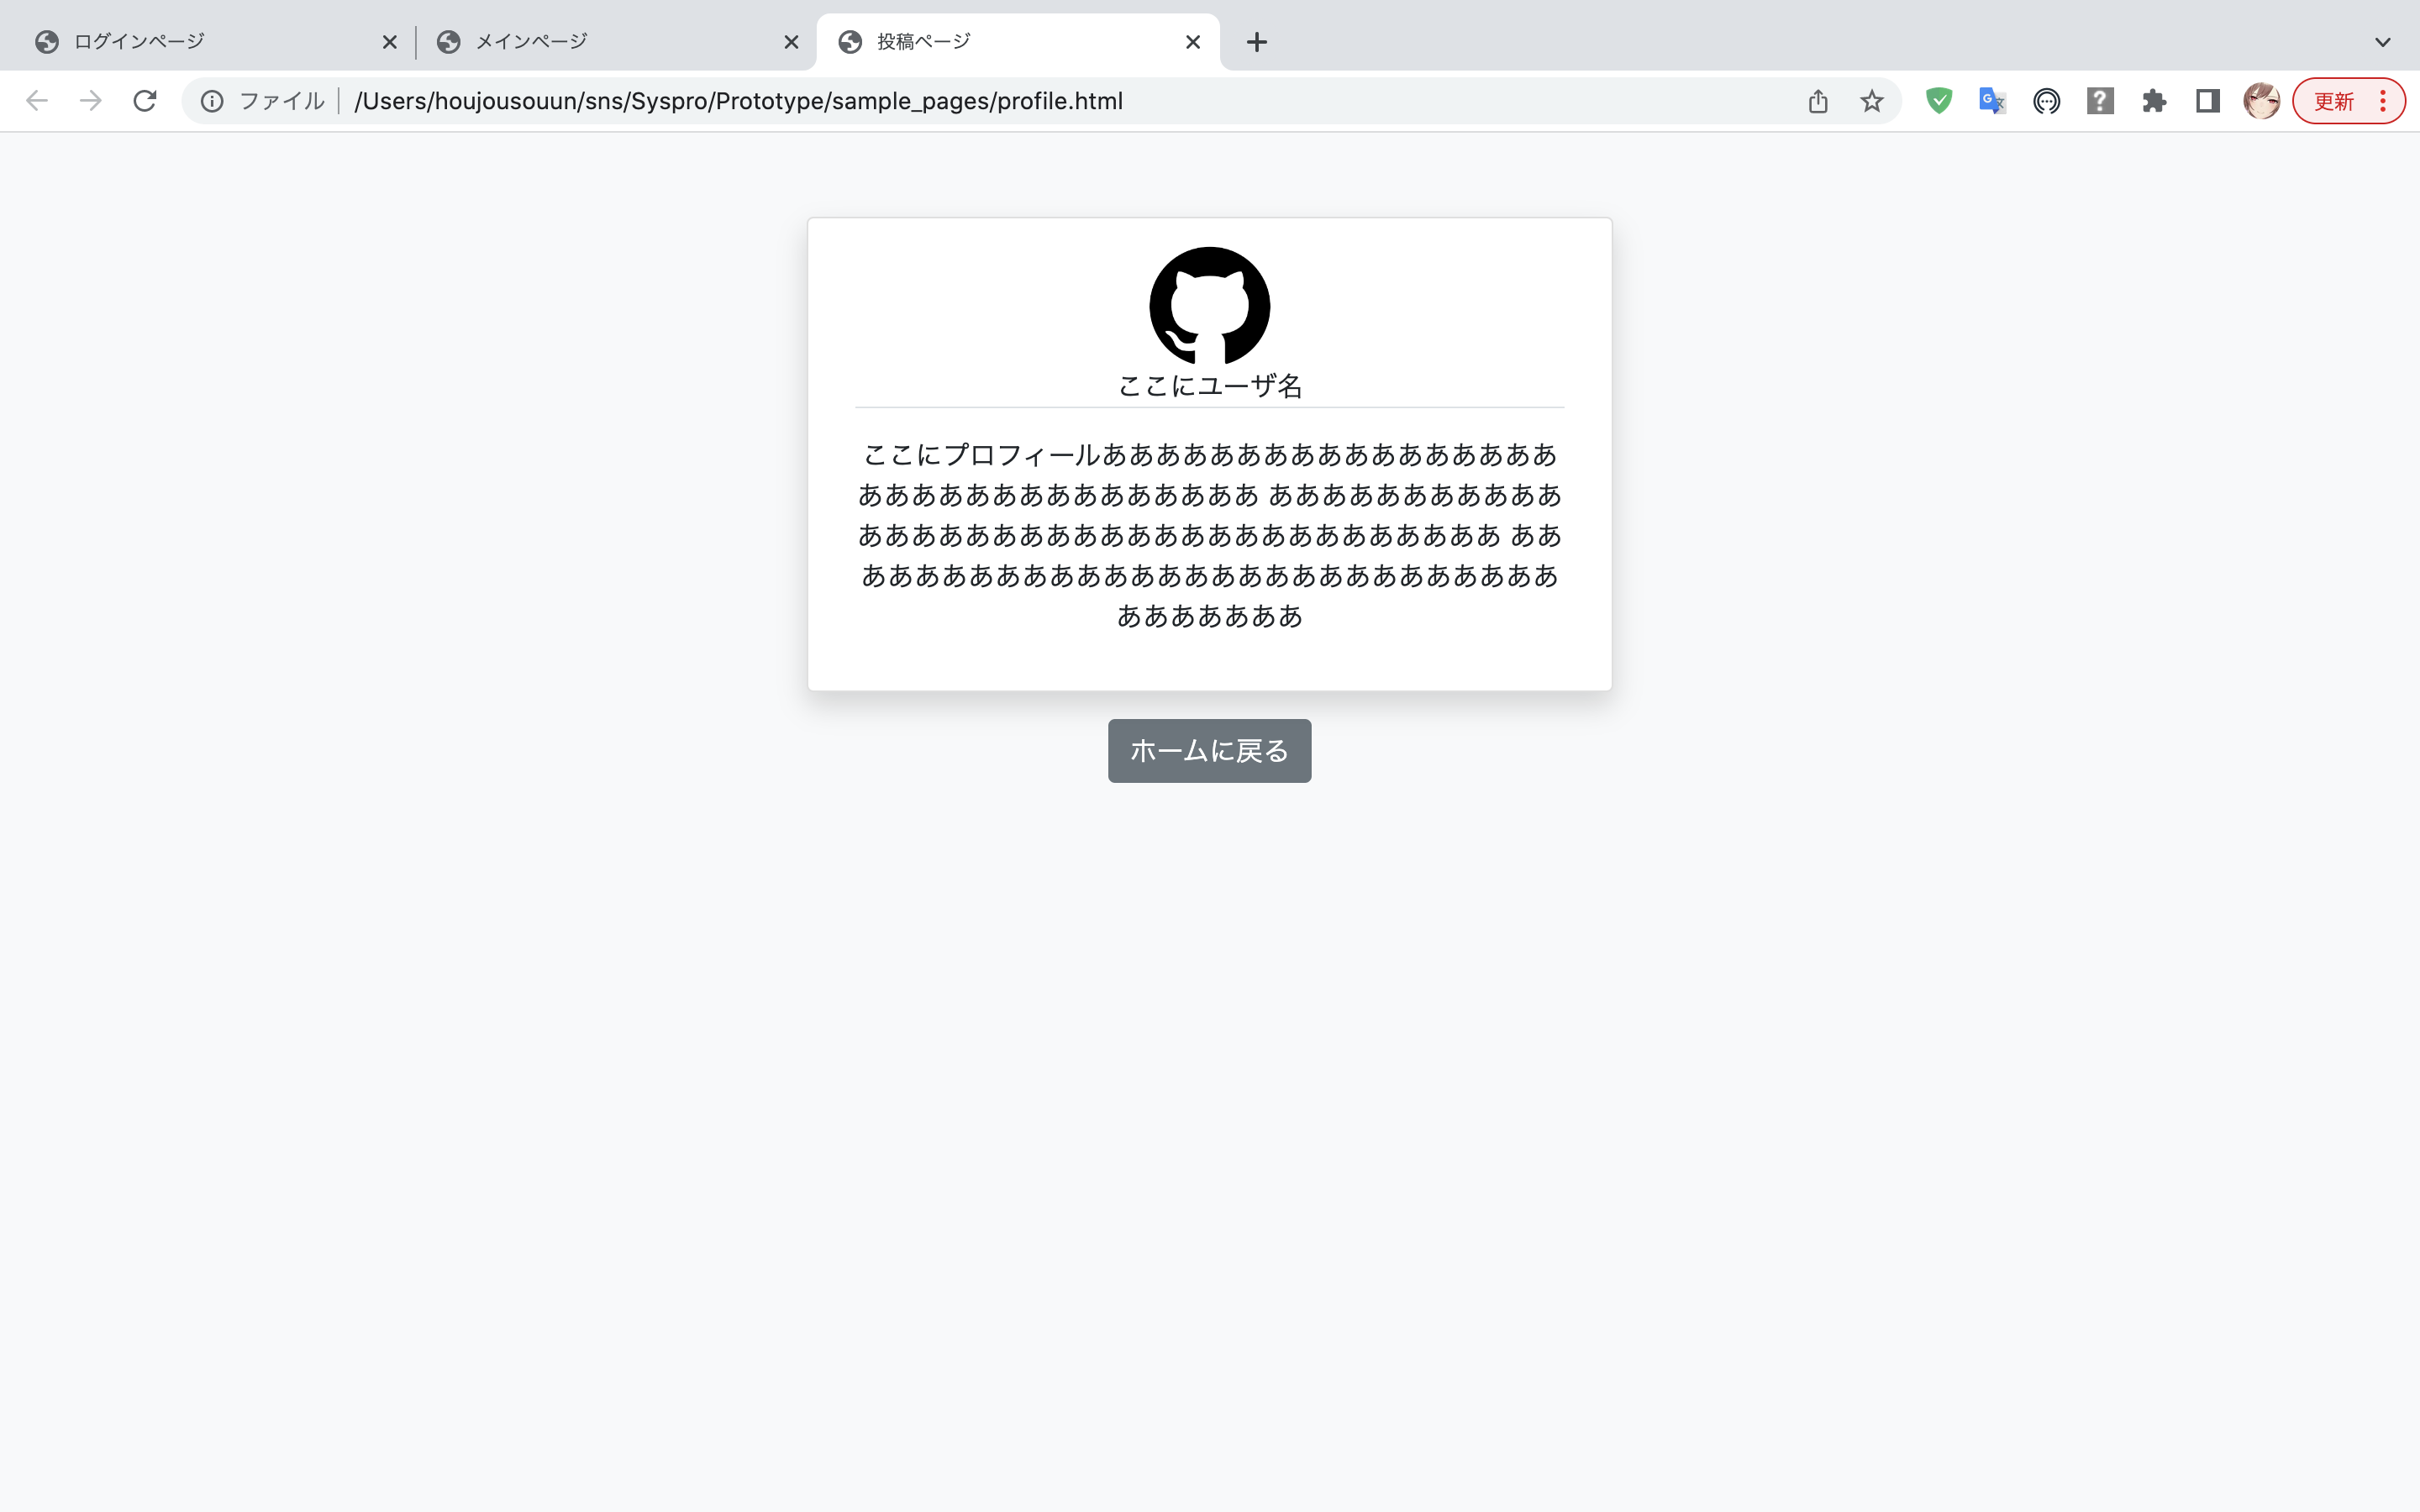
\includegraphics[scale=0.3,clip]{pictures/profile.png}
        \end{center}
    \end{figure}

    \begin{figure}[H]
        \begin{center}
            \caption*{searchForm.html}
            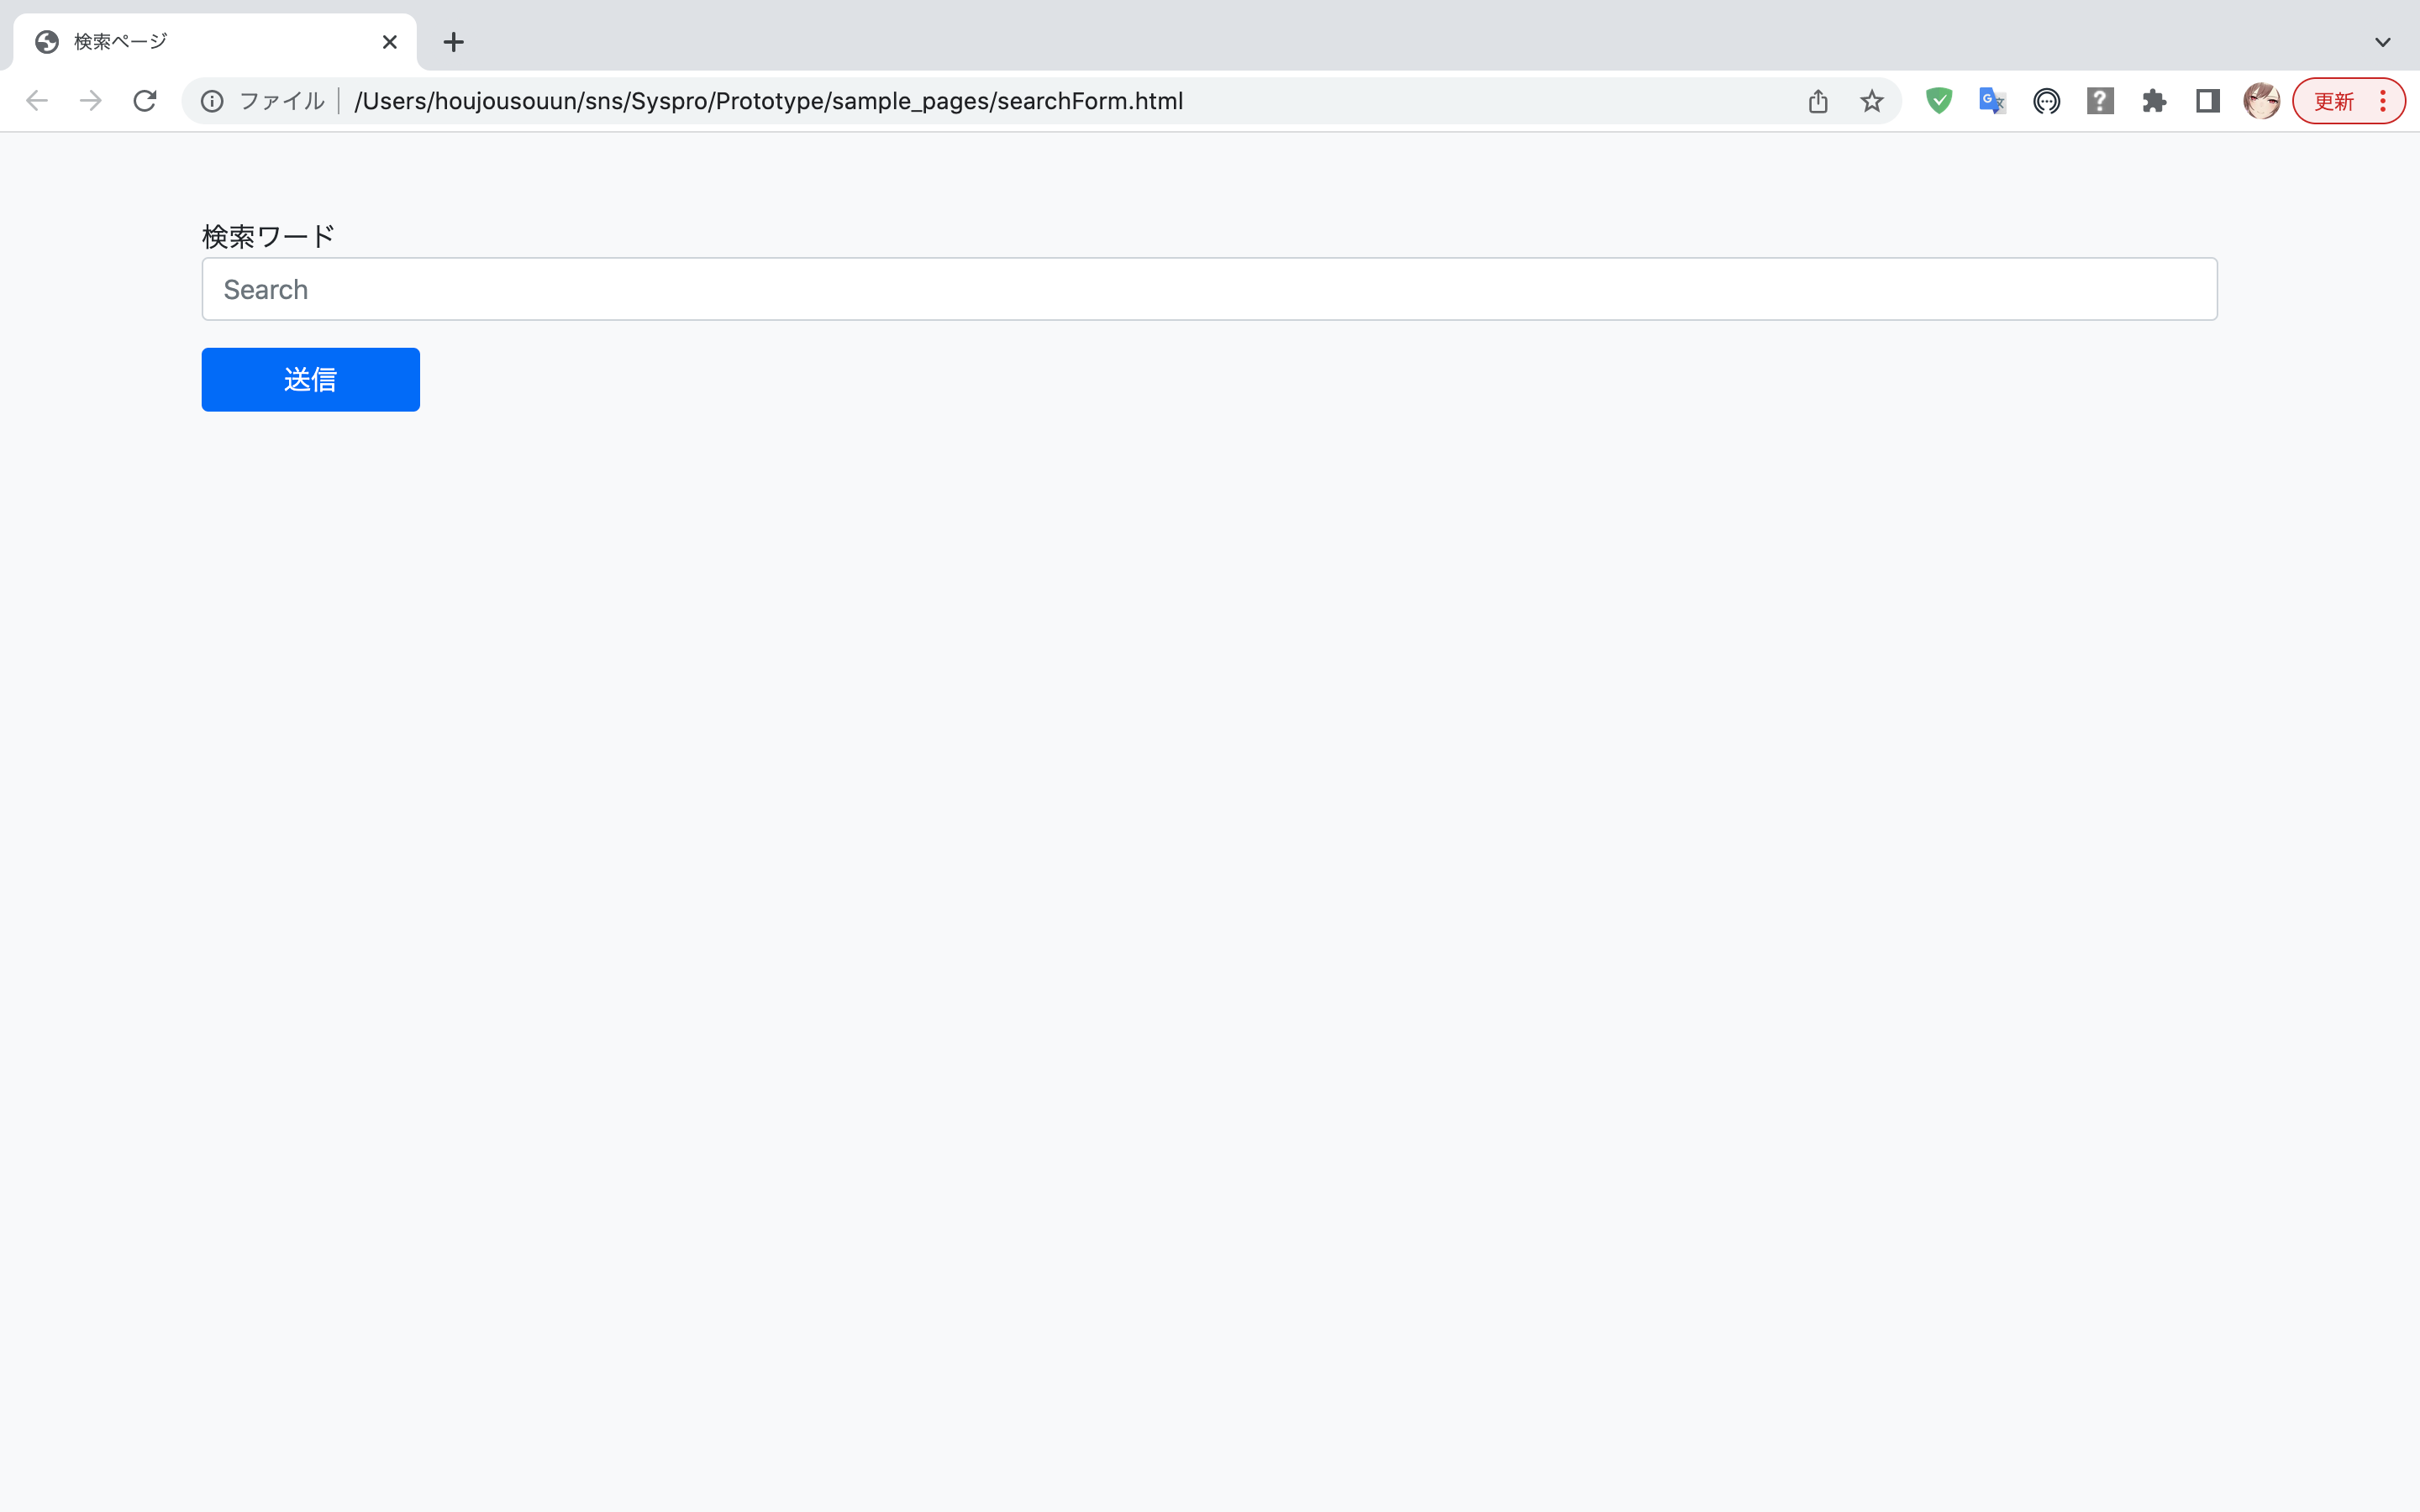
\includegraphics[scale=0.3,clip]{pictures/searchForm.png}
        \end{center}
    \end{figure}

    \begin{figure}[H]
        \begin{center}
            \caption*{bookForm.html}
            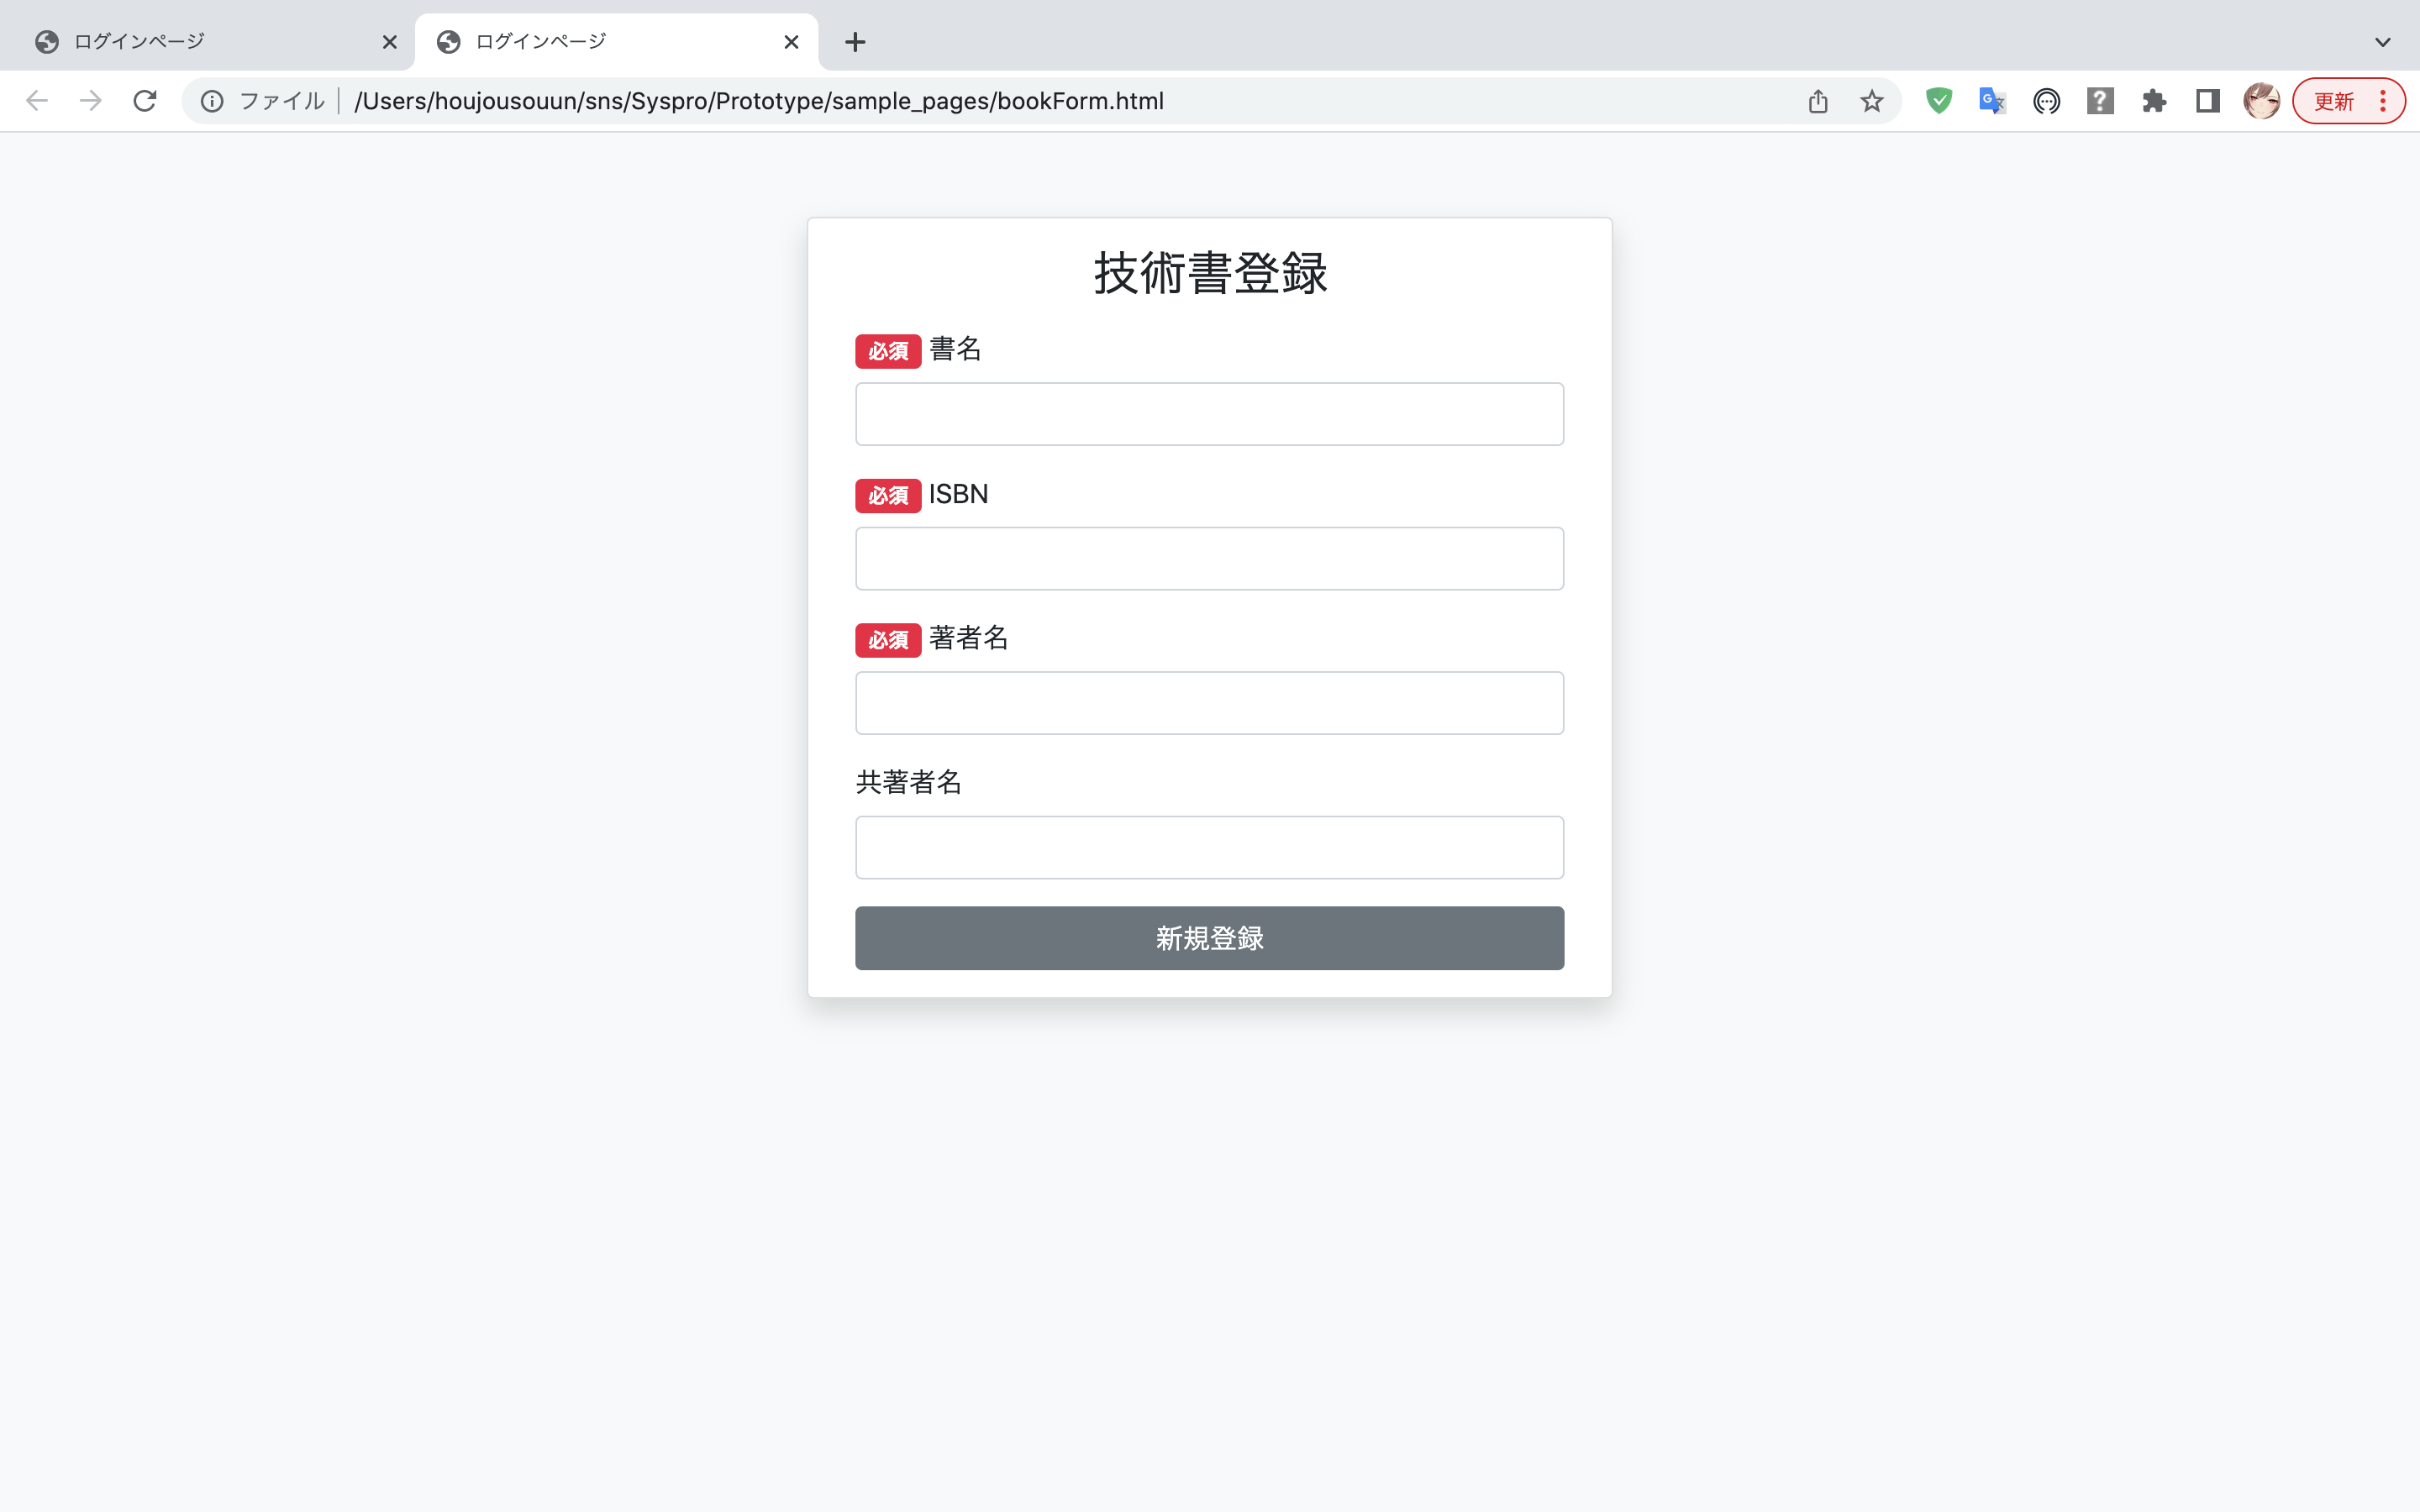
\includegraphics[scale=0.3,clip]{pictures/bookForm.png}
        \end{center}
    \end{figure}

    \begin{figure}[H]
        \begin{center}
            \caption*{commentForm.html}
            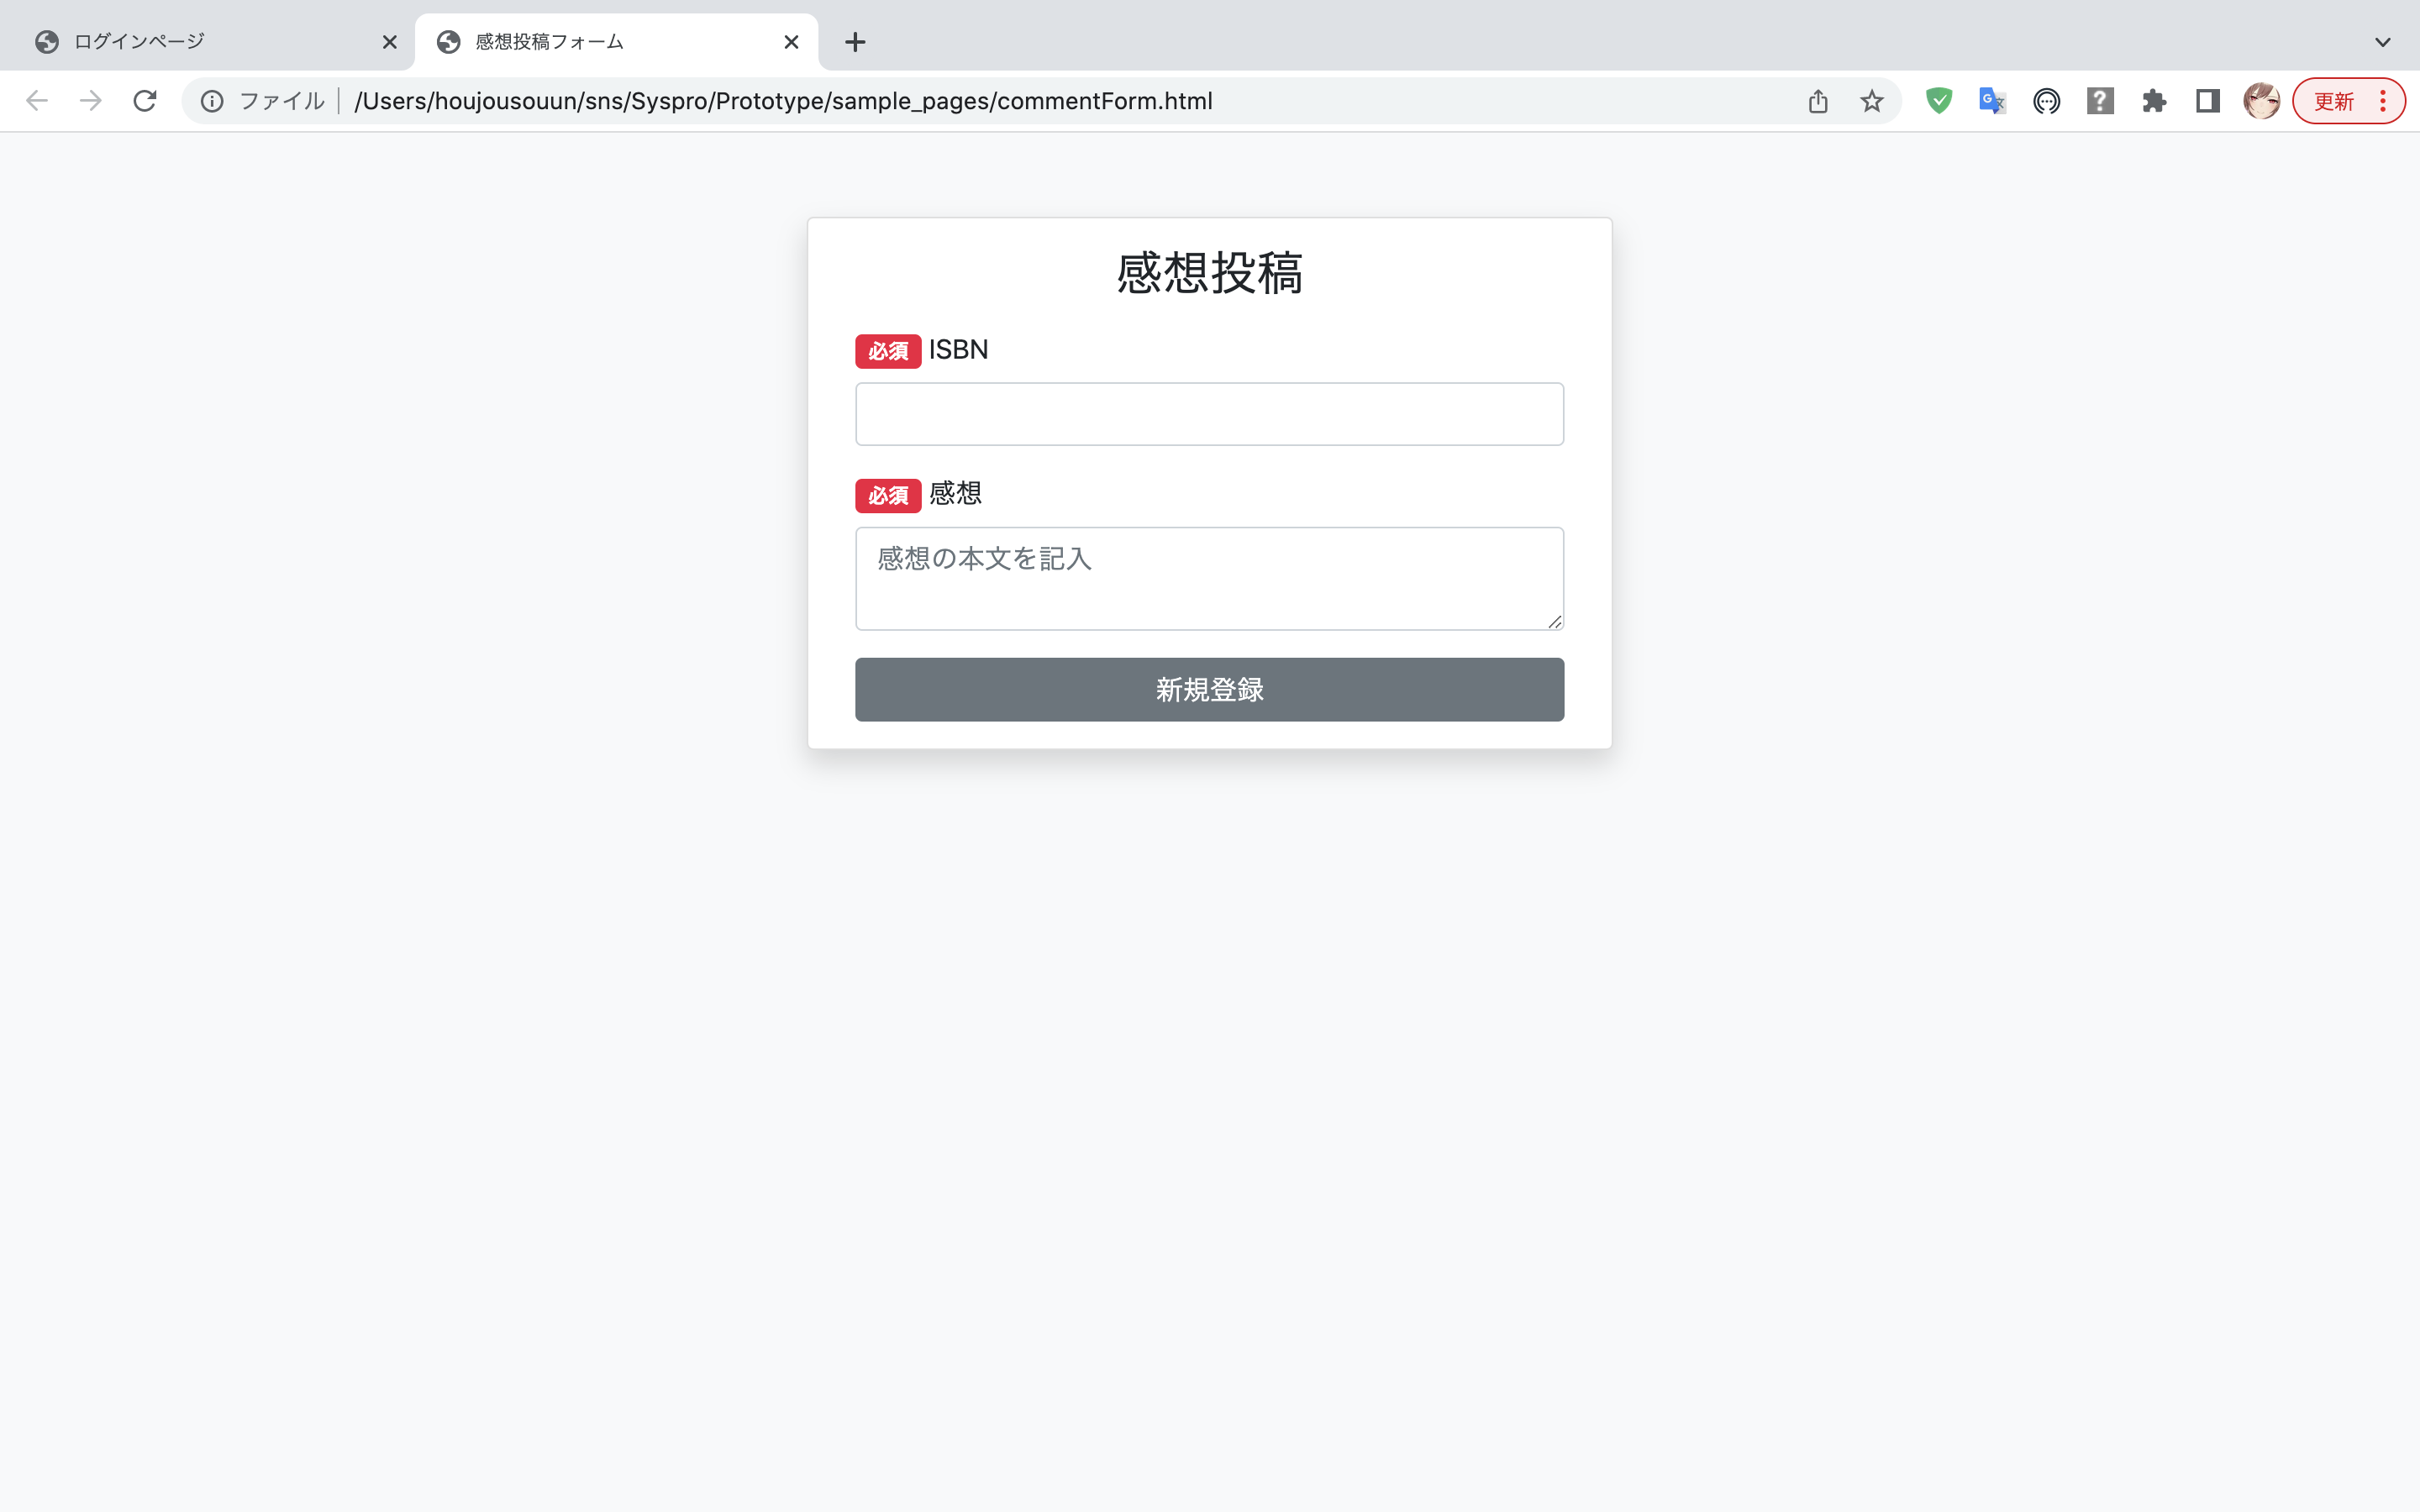
\includegraphics[scale=0.3,clip]{pictures/commentForm.png}
        \end{center}
    \end{figure}


    \section*{概念クラス図}
    \subsection*{\rm{作成者:實藤(フロントエンド担当)}}
    \begin{figure}[H]
        \begin{center}
            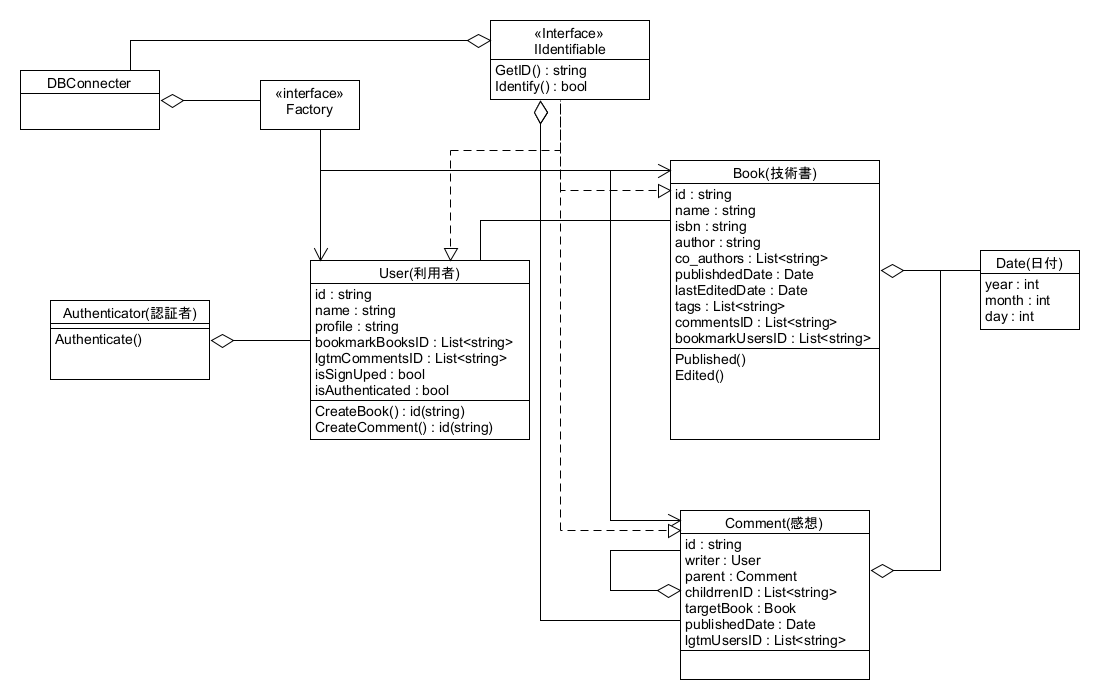
\includegraphics[scale=0.4,clip]{pictures/SysPro-ModelClassImage.png}
        \end{center}
    \end{figure}

    \newpage

    \section*{詳細クラス図}
    \subsection*{\rm{作成者:實藤(フロントエンド担当)}}
    \begin{figure}[H]
        \begin{center}
            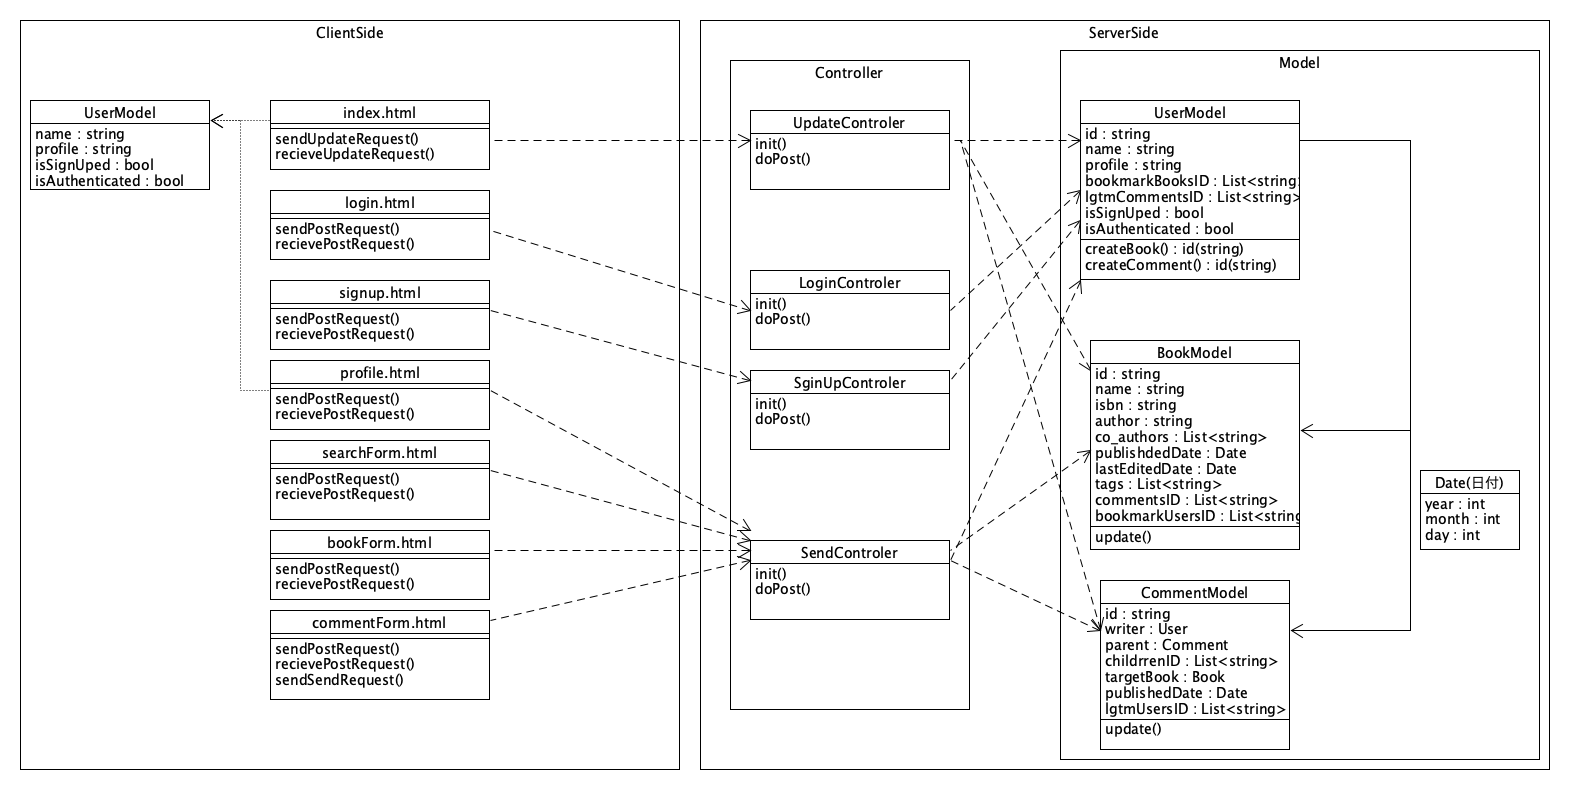
\includegraphics[scale=0.3,clip]{pictures/MVC.png}
        \end{center}
    \end{figure}

    \newpage

    \section*{シーケンス図}
    \subsection*{\rm{作成者:穂積(バックエンド担当)}}
    \begin{figure}[H]
        \begin{center}
            \caption*{アカウントを登録する}
            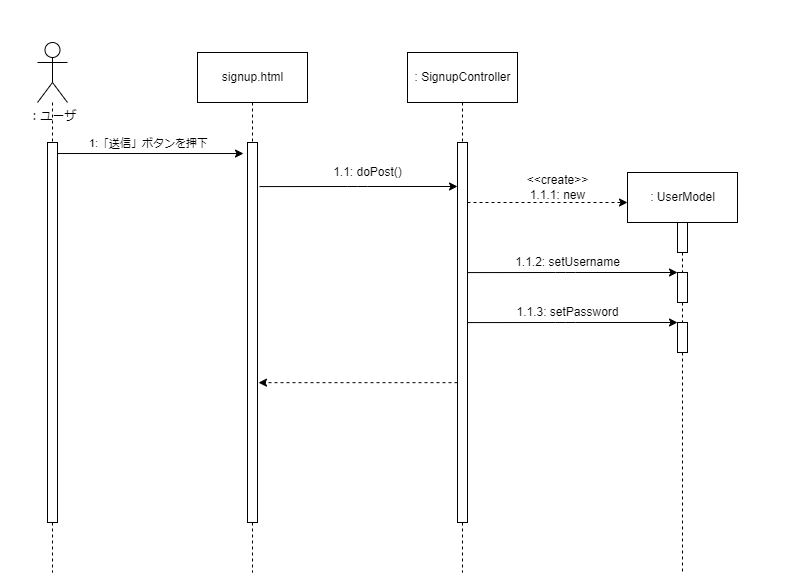
\includegraphics[scale=0.6,clip]{pictures/sequence-graph/signup.png}
        \end{center}
    \end{figure}

    \begin{figure}[H]
        \begin{center}
            \caption*{アカウントにログインする}
            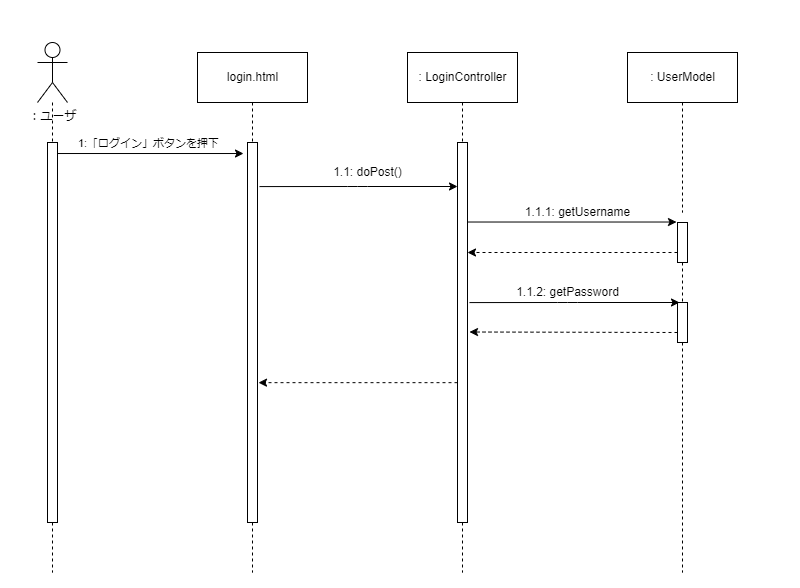
\includegraphics[scale=0.6,clip]{pictures/sequence-graph/login.png}
        \end{center}
    \end{figure}

    \begin{figure}[H]
        \begin{center}
            \caption*{技術書に関して投稿する}
            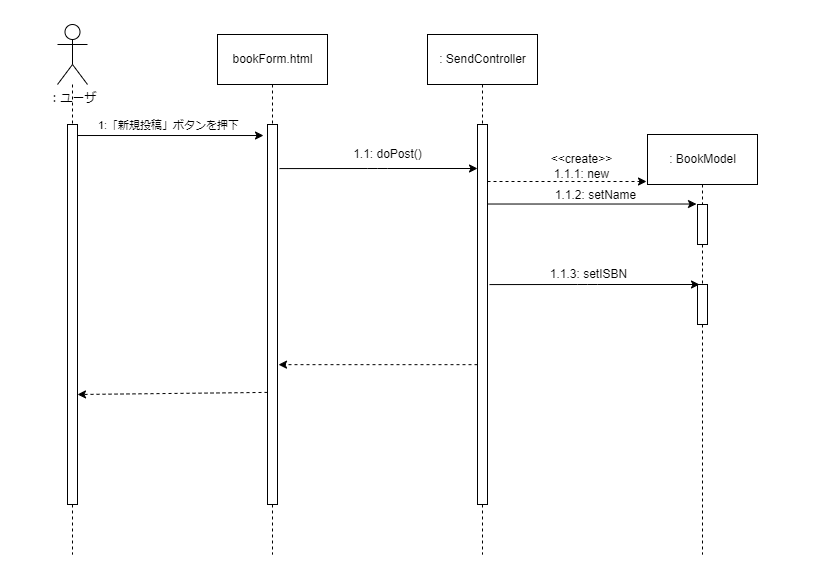
\includegraphics[scale=0.6,clip]{pictures/sequence-graph/sendAboutBook.png}
        \end{center}
    \end{figure}

    \begin{figure}[H]
        \begin{center}
            \caption*{技術書に関する投稿を閲覧する}
            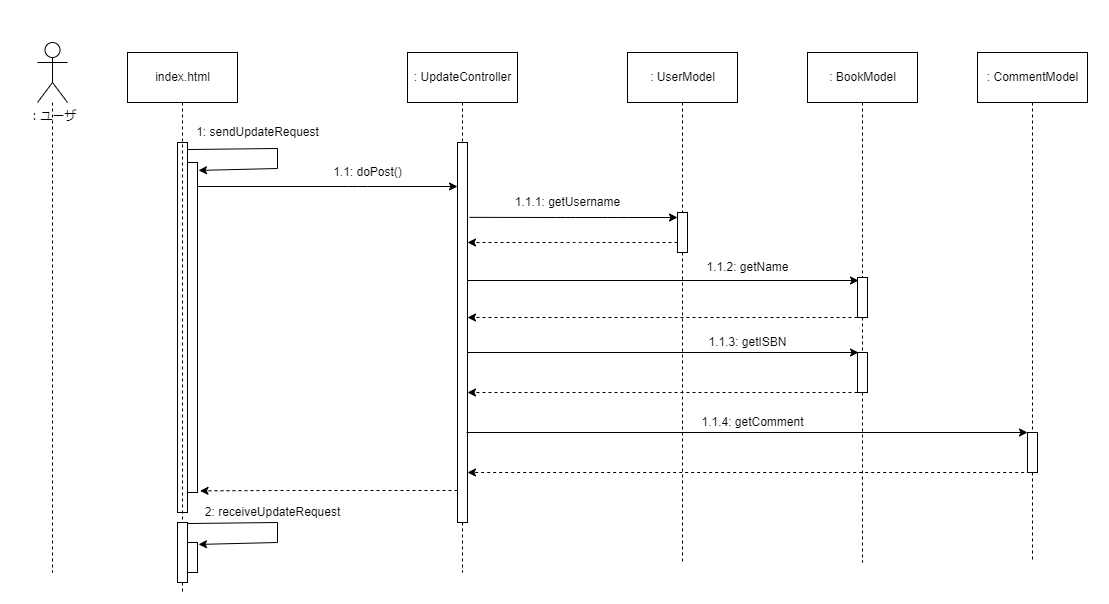
\includegraphics[scale=0.45,clip]{pictures/sequence-graph/watchMessages.png}
        \end{center}
    \end{figure}

    \begin{figure}[H]
        \begin{center}
            \caption*{他人の投稿に対して反応する}
            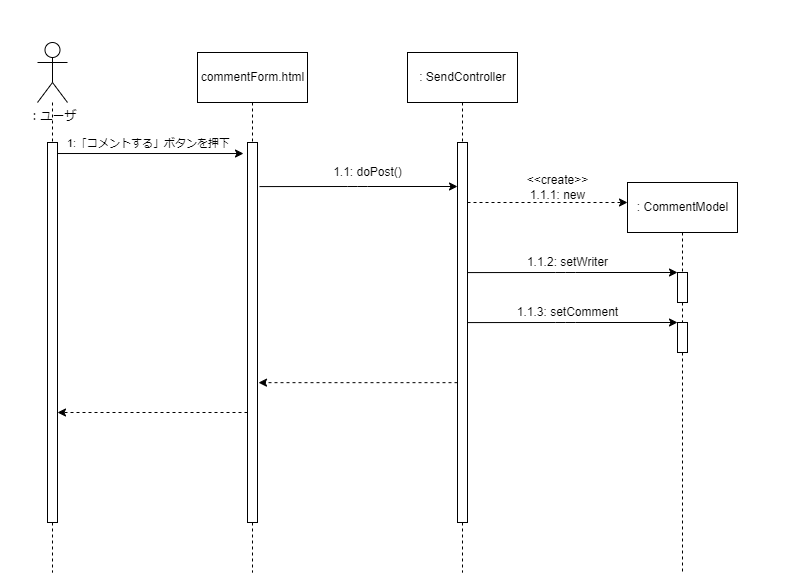
\includegraphics[scale=0.6,clip]{pictures/sequence-graph/reaction.png}
        \end{center}
    \end{figure}

    \begin{figure}[H]
        \begin{center}
            \caption*{技術者を検索する}
            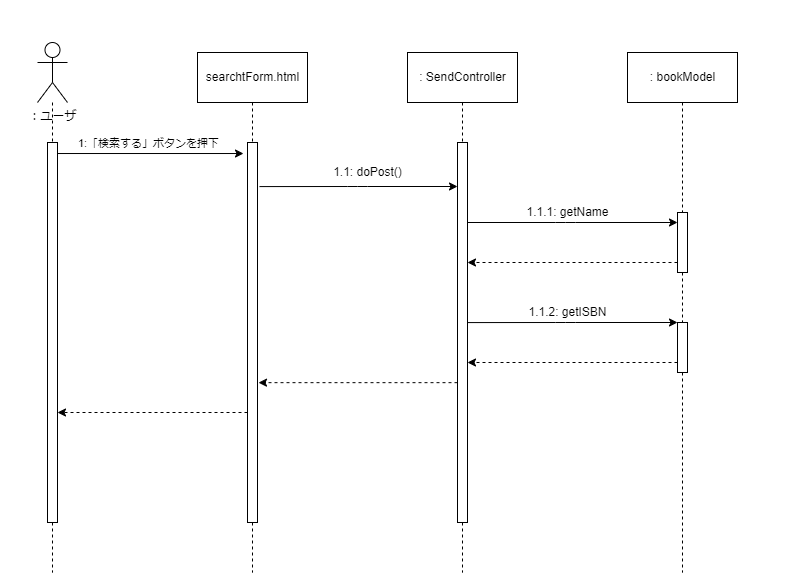
\includegraphics[scale=0.6,clip]{pictures/sequence-graph/searchBook.png}
        \end{center}
    \end{figure}

\end{document}